\chapter{CW-Cache:设计与分析}
\label{chp:cw-cache}

\par 根据第~\ref{chp:motivation}章的实验和第~\ref{chp:column-aware}章对Column-aware方案的分析,我们了解到方案的一些需求:
\begin{itemize}
    \item 方案需要根据数据表中各个列的热度(访问频率)决定哪一些列需要被复制,复制多少份。
    \item 如果复制后的列的副本分开存储,执行SQL查询任务时会引起shuffling,且shuffling会对任务执行时间产生不可小觑的影响,我们设计的方案需要尽力避免。
    \item 方案应该尽可能减少上层计算框架和中间缓存系统的耦合度,缓存系统利用的额外信息要尽可能少。
\end{itemize}

\par 我们给系统取名为CW-Cache,CW是Column-wise两个单词的首字母,取自它实现列级别负载均衡的目标。吸取Column-wise方案的经验教训,我们提出了另一个用于CW-Cache系统的方案,我们称这个方案为“Bundle-K”,正如字面意思所示,我们经过统计后将数据表中的各个列按照热度(访问频率)进行排序,然后“捆绑”前$K$个列进行复制。在执行查询任务的时候,如果查询任务涉及的所有列均在这复制出来的前$K$个列中,那么就由副本为查询任务提供数据,否则就由原表为任务提供数据。那么问题来了,这个$K$取多少合适呢?即使确定了$K$,那么这前$K$列要复制多少份比较合适呢?这并不是拍脑袋就能想出来的,接下来我会对此方案进行数学建模与分析,用公式进行推导。

\section{问题建模}
\label{sec:bundle-k-model}

\subsection{符号定义}

\par 这里我们对一张数据表内的列级别的共同\emph{访问模式}进行描述。假设这张表共有$n$列,记为 $\left\{c_{0}, c_{1}, \dots, c_{n-1}\right\}$ ,它们所占空间的归一化分别是 $\left\{s_{0}, s_{1}, \dots, s_{n-1}\right\}$ ,则 $\sum_{i=0}^{n-1} s_i = 1$ ,一些查询任务会访问一组特定的列,我们称这一组列是一个共同访问模式。假设有$m$个共同访问模式 $T = \left\{t_{0}, t_{1}, \dots, t_{m-1}\right\}$ ,对于某一个特定的访问模式$t_i$,它的热度$p_i$代表了有这个访问模式的查询任务的数量,$ts_i$是这个访问模式中所有列的大小之和。这$m$组共同访问模式的负载分别是 $\left\{l_{0}, l_{1}, \dots, l_{m-1}\right\}$ ,其中 $l_i = p_i ts_i$ 。

\par 记$k$为复制的最热门的列的数量,$S_k$是这复制的$k$列组成的副本能够覆盖的访问模式的集合,那么所有的访问模式就被分成了两组,$S_k$和$T-S_k$。记$L_h$和$L_c$分别是$S_k$和$T-S_k$承担的总负载,则有 $L_h=\sum_{i \in S_{k}} l_{i}$ 以及 $ L_c = \sum_{i \notin S_{k}} l_{i}$。

\par 假设我们的集群有$N$台服务器,我们的目标是找到$k$和副本的数量$r$来最小化任意一台服务器的\emph{负载的方差}和\emph{复制的代价}。

\subsection{目标}
\par 记$X$是任意一台服务器的负载,那么有:

\begin{equation}
    X=a_{0} \frac{L_{h}}{r}+a_{1} L_c,
\end{equation}

\par 其中$a_0$ 和 $ a_1$ 是二元随机变量,表示一个副本/原表是否被放置在这台机器上。由于我们将副本和原表随机放置在集群中,$a_0$ 和 $ a_1$ 服从伯努利分布且相互独立,因此我们能够得出:

\begin{equation}
\begin{split}
\operatorname{Var}(X)&=\frac{L_{h}^{2}}{r^{2}}\frac{r}{N}\left(1-\frac{r}{N}\right)+L_{c}^{2}\frac{1}{N}\left(1-\frac{1}{N}\right) \\
& = \frac{1}{N}\left(\frac{L_{h}^{2}}{r}+L_{c}^{2}\right) - \frac{1}{N^2}\left( L_h^2 + L_c^2\right)
\end{split}
\end{equation}

\par 记 $C$ 为复制的代价,即缓存这些副本占用的内存空间,我们有:

\begin{equation}
    C = r \sum_{i=0}^{k-1} s_i
\end{equation}

\par 我们的目标是使得负载的方差与复制的代价的加权和最小化。假设权重为 $w$,那么:

\begin{equation}
\label{eq:obj}
\begin{aligned}
\min \quad & \frac{1}{N}\left(\frac{L_{h}^{2}}{r}+L_{c}^{2}\right) - \frac{1}{N^2}\left( L_h^2 + L_c^2\right) + w\times r \sum_{i=0}^{k-1} s_i\\
\textrm{s.t.} \quad & k \in \{1, \cdots, n\}\\
& r \in \{1, \cdots, N\}    \\
\end{aligned}
\end{equation}

\section{算法}
\label{sec:alg}

\par 我们可以通过遍历所有可能的值,即从1到n,来寻找最佳的$k$。具体来说,对于每一个可能的$k$值,我们那更新$S_k$来计算$L_h$ 和 $L_c$,接着我们计算当前的$k$值下最优的$r$值。用$f(r)$并表示目标函数,我们能够发现:

\begin{equation}
f'(r) = - \frac{L_h^2}{Nr^2} + w\sum_{i=0}^{k-1} s_i
\end{equation}
\par 当 $f'(r) = 0$,可以得到:
\begin{equation}
\label{eq:r}
r = \sqrt{\frac{L_h^2}{N w \sum_{i=0}^{k-1} s_i}},
\end{equation}

\par 在这个例子中,我们的目标函数$f(r)$能够求到最小值。

\begin{algorithm}[tb]
	\caption{Find optimal $k$ and $r$}
	\label{alg:algo}
	\small
	\begin{algorithmic}[1]
		\Statex{-- $T$: 所有的共同访问模式}
		\Statex{-- $l[0\cdots m-1]$: $m$ 个访问模式的负载}
		\Statex{-- $w$: 最小化目标函数(等式~\ref{eq:obj})中的权重}
		
		\Function{UpdateSk}{$k, S_k, O_k$} \Comment{update $S_k$}
		\ForAll{$t \in O_k$}
		\If{$k$ hottest columns contain $t$}
		\State{move $t$ from $O_k$ to $S_k$}
		\EndIf
		\EndFor
		\EndFunction
		
		\Function{FindOpt}{}
		\State{$S_k \gets \{\}$}\Comment{初始化 $S_k$}
		\State{$O_k \gets T$}\Comment{初始化 $T - S_k$}
		\State{$opt\_k \gets -1$}\Comment{初始化最优值 $k$}
		\State{$opt\_r \gets -1$}\Comment{初始化最优值 $r$}
		\State{$opt\_obj \gets + \infty$}\Comment{初始化最优目标}
		\ForAll{$k \in \{1, \cdots, n\}$}
		\State{$\Call{UpdateSk}{k, S_k, O_k}$}
		\State{$L_h \gets \sum_{i \in S_{k}} l_{i}$}
		\State{$L_c \gets \sum_{i \notin S_{k}} l_{i}$}
		\State{$r \gets$ get integer r using equation \ref{eq:r}}
		\State{$r \gets \min\{N, r\}$}\Comment{$r \leq N$}
		\State{$obj \gets$ calculate objective in equation \ref{eq:obj}}
		% \State{$l' \gets \Call{CalcLat}{1, k} + \Call{CalcLat}{k + 1, n}$}
		\If{$obj < opt\_obj$}\Comment{更新 $k, r, obj$}
		\State{$opt\_k \gets k$}
		\State{$opt\_r \gets r$}
		\State{$opt\_obj \gets obj$}
		\EndIf
		\EndFor
		\State{\Return $opt\_k, opt\_r$}
		% \State{$l' \gets \min_{k \in \{2, \cdots, n - 1\}} \Call{CalcLat}{1, k} + \Call{CalcLat}{k + 1, n}$}
		% \If{$l - l' > w\beta$} \Comment{estimate regret}
		% \State{\Return \texttt{true}}
		% \Else
		% \State{\Return \texttt{false}}
		% \EndIf
		\EndFunction
	\end{algorithmic}
\end{algorithm}


\par 算法~\ref{alg:algo}展示了求解最优的$k$ 和 $r$的过程。时间复杂度为$O(n + m)$,其中$n$是列的数量而$m$是访问模式的数量。

\par 算法~\ref{alg:algo}中 最耗时的步骤是对每一个$k$值更新$S_k$,把所有的访问模式$T$排个序是可选的降低开销的方法。具体来说,对于访问模式$t_i$,记$e_i$是其热门度最低的列,我们把$T$中的$m$个访问模式按照它们热门度最低的列的热门度进行排序$\left\{e_{0}, e_{1}, \dots, e_{m-1}\right\}$。这样,随着$k$的增加,排序后的$T$中的访问模式就会依次被覆盖。

\par 算法~\ref{alg:update}展示了当$T$被排好序后,更新$S_k$的过程。基于排序后的$T$来搜索最佳的$k$ 和 $r$,时间复杂度是$O(n + m)$,假设此排序过程的时间复杂度是$O(m\log{m})$(例如快速排序),那么总的时间复杂度是$O(m\log{m} + n)$。

\begin{algorithm}[tb]
	\caption{Update $S_k$ for sorted $T$}
	\label{alg:update}
	\small
	\begin{algorithmic}[1]
		\Function{UpdateSk}{$k, S_k, O_k$}
		\ForAll{$t \in O_k$}
		\If{$k$ hottest columns contain $t$}
		\State{move $t$ from $O_k$ to $S_k$}
		\Else
		\State{\Return}
		\EndIf
		\EndFor
		\EndFunction
		
	\end{algorithmic}
\end{algorithm}

\section{通过列的热门度估算共同访问模式}
\label{sec:estimate-patern}
\par 上一节我们的建模引入了列的共同访问模式,对于一张表来说,如果这张表有$N$列,理论上它能产生$2_N$种访问模式,当$N$比较大的时候,访问模式的数量是我们无法接受的。要想获得访问模式,一种方法是Master在内存中维护每一种出现过的访问模式的计数器,即统计它们的热度信息。问题是对于列比较多的表,要想维持这么多计数器是非常消耗内存资源的,内存资源本就紧缺,应该用在刀刃上。于是我们设想,能否利用列的热度信息来推测访问模式的热度?下面我们进行数学建模并加以实验验证。

\subsection{符号定义}

\par 对于某张数据表,假设它有$n$个列 $\left\{ c_{1}, c_{2}, \dots ,c_{n} \right\} $,它们的归一化的体积为$\left\{ s_{1}, s_{2}, \dots ,s_{n} \right\} $,那么 $\sum_{i=1}^{n}s_i = 1$ 。假设现在有$m$个查询任务访问这些列。这些列的热度记为 $ P = \left\{ p_{1}, p_{2}, \dots, p_{n} \right\} $,它们的负载是$ L = \left\{ l_{1}, l_{2}, \dots, l_{n} \right\} $,其中 $l_i = p_i s_i$。用$L_a$来表示负载的总和,那么我们有 $L_a = \sum_{i=1}^{n}l_i$。

\par 在~\ref{sec:bundle-k-model}节中,我们假设确定复制前$k$个最热门的列,然后计算呢它们能覆盖的访问模式,并把它们的负载累加起来得到$L_h$。在本节中,我们放弃详细的访问模式的信息,仅仅通过列的热度信息来估计$L_h$。

\subsection{推测}

\par 我们可以根据列的热度随机生成查询任务来估算访问模式的分布。对于一个查询任务,它访问列$c_i$的可能性是$\frac{p_i}{m}$。假设查询任务是否访问每一个列是相互独立的,那么$n$个列被一个查询任务访问的概率是$B = \left\{\frac{p_{1}}{m}, \frac{p_{2}}{m}, \dots, \frac{p_{n}}{m}\right\}$。

\par 为了估计访问模式的分布,首先我们给每一个列分配等同于它们热度的“配额”,接着我们按照$B$中的比例生成查询任务,直到所有配额用尽。基于这些生称的查询任务和访问模式,我们能够研究$L_h$ 和 $k$ 之间的关系。

\par \noindent \textbf{测量实验1} \quad 首先我们通过TPC-DS标准测试程序测试了上文提出的方法。对于每一张表,我们统计每个列的热度以及访问过该表的查询任务的数量。接着我们生成查询任务,通过蒙特卡罗方法估计$k$取不同的值下的$L_h$。为了简化问题,我们假设所有的列的大小相等。

\par 图~\ref{fig:mc_gt}展示了TPC-DS中三张具有代表性的数据表中列的热度及归一化的$L_h$,即 $\frac{L_h}{L_a}$ 和 $k$之间的关系。为估算$L_h$,我们对比了蒙特卡罗方法(Monte Carlo method(MC))和实际情况(ground truth(GT))。从图~\ref{fig:mc_gt}上可以看出,两种方法对应的曲线吻合程度是比较高的,也就是说,就$L_h$ 和 $k$之间的关系而言,我们可以通过随机生成查询任务这种方法来估算访问模式的分布。


\begin{figure}[]
    \centering
    \begin{subfigure}[t]{0.5\textwidth}
        \centering
        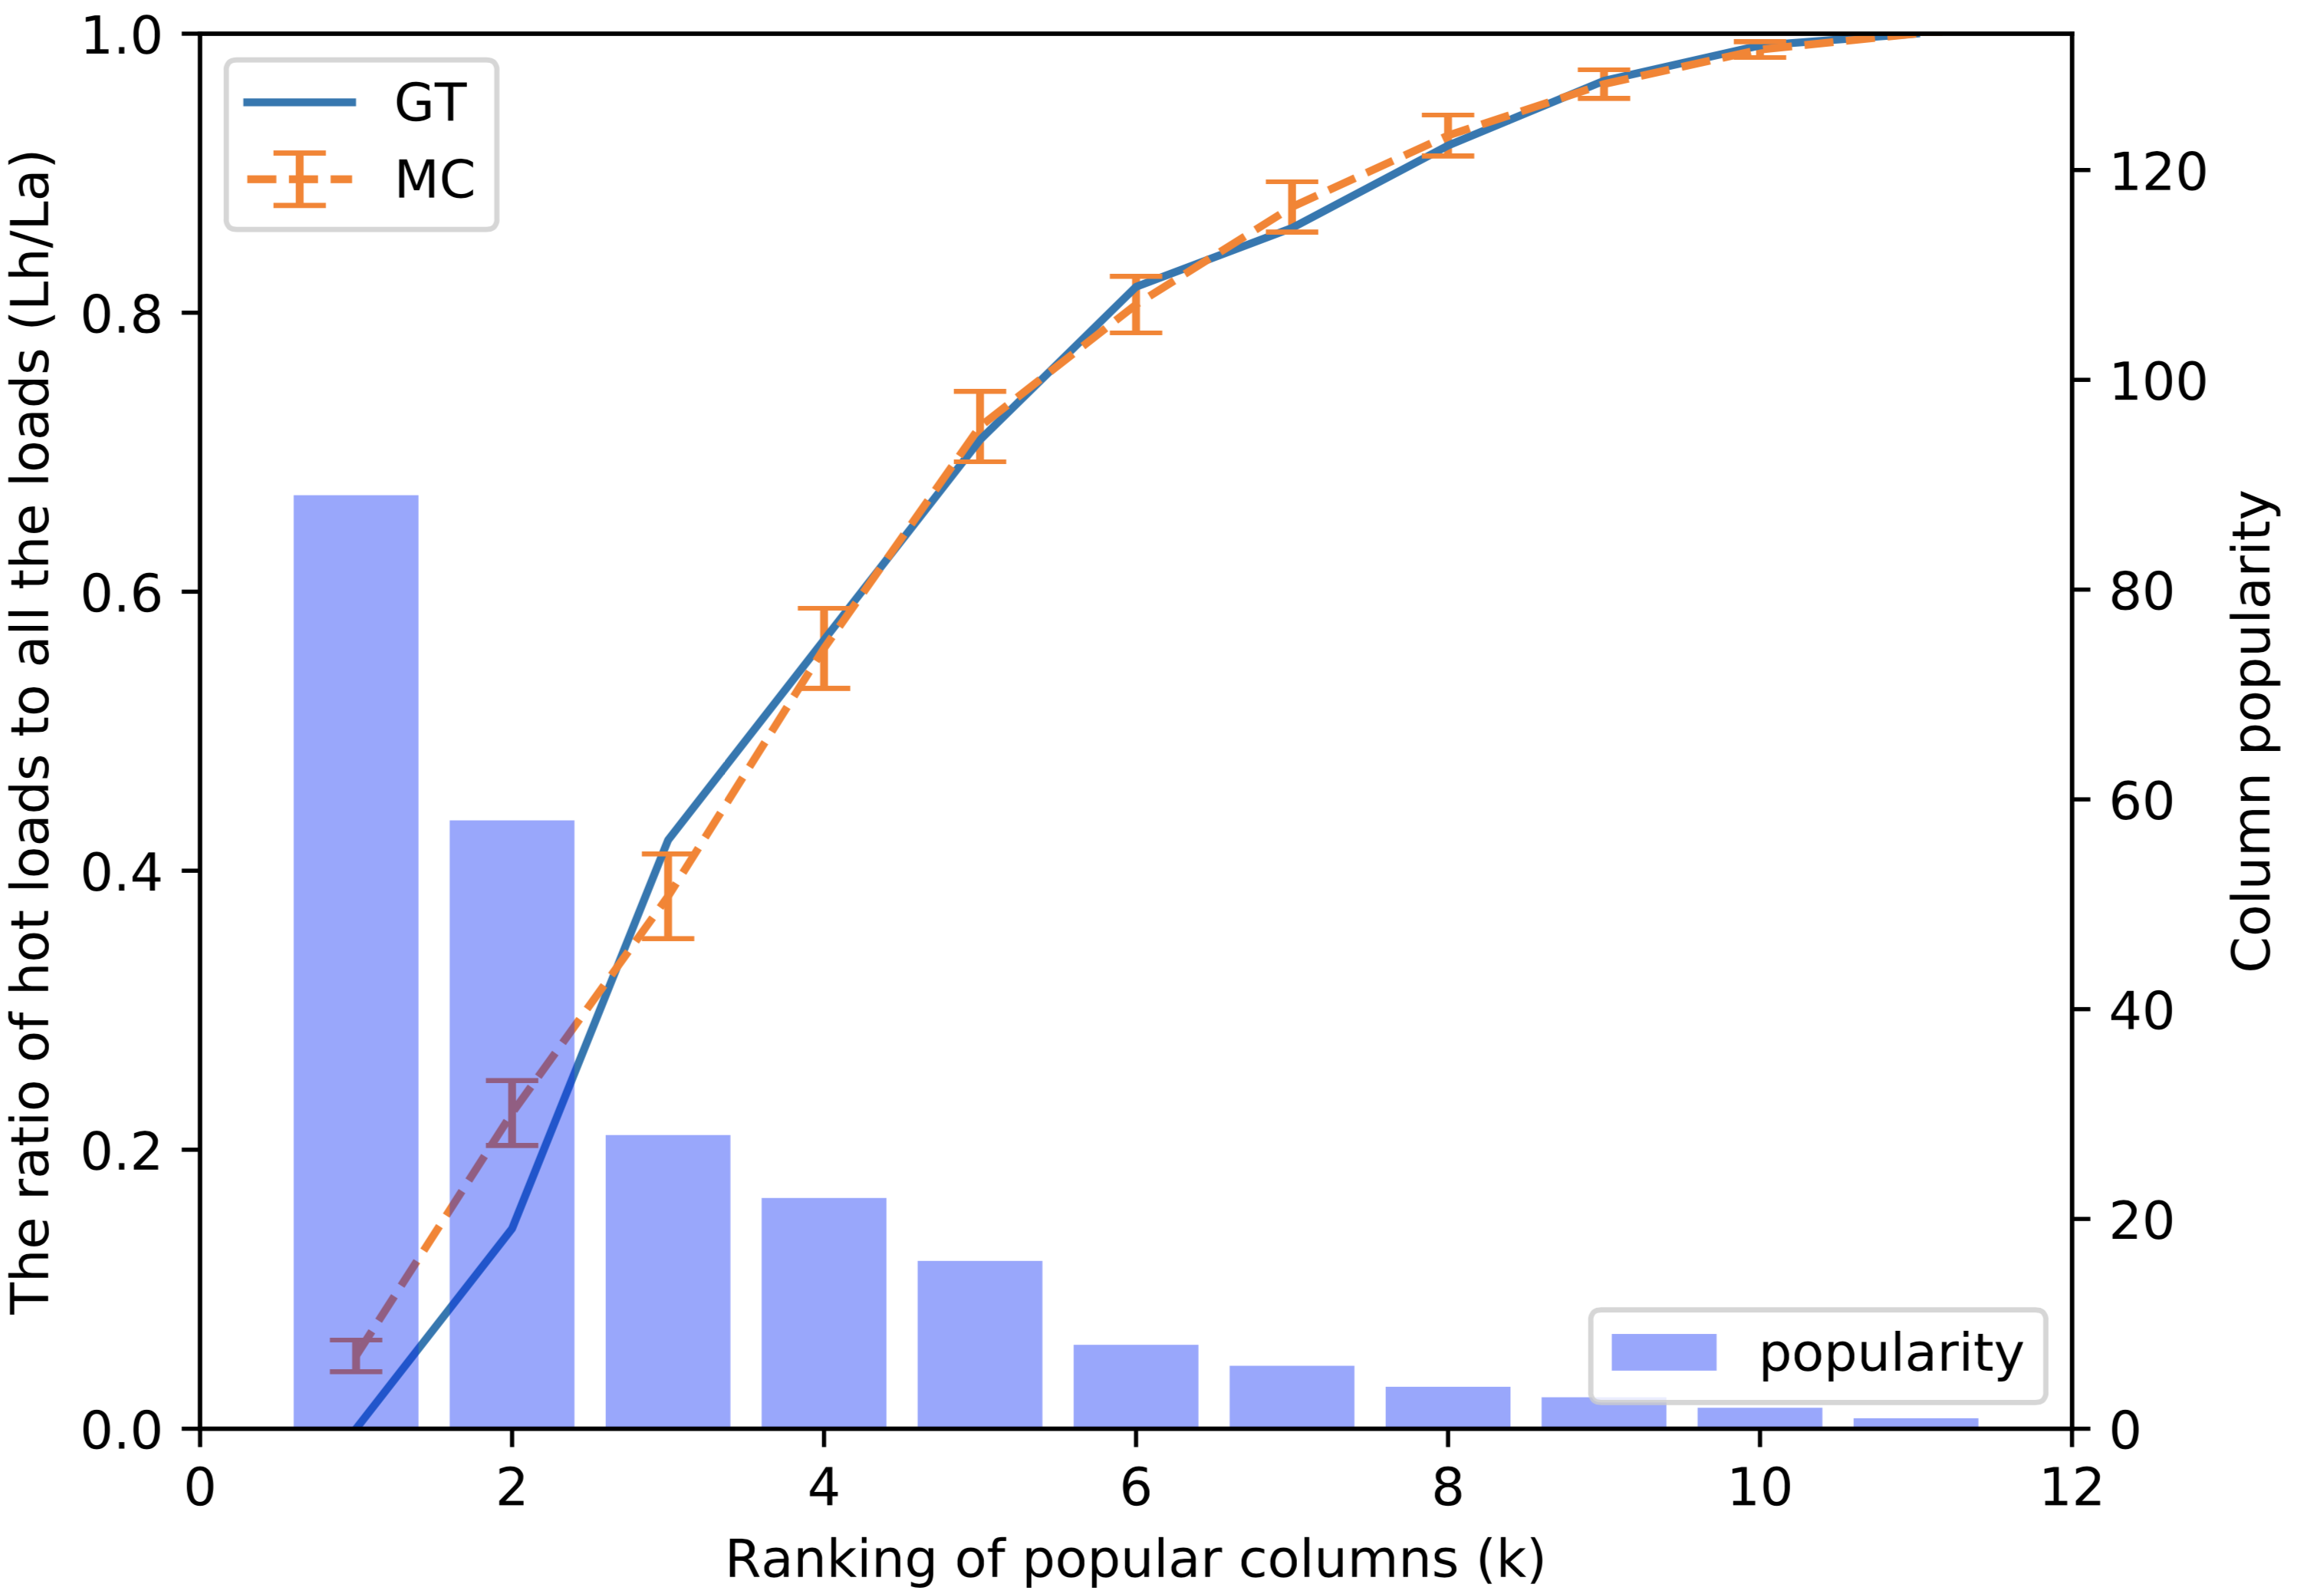
\includegraphics[width=1\textwidth]{img/cw-cache/ca_date_dim}
        \caption{TPC-DS中的 $data\_dim$ 表}
        \label{fig:ca-dd}
    \end{subfigure}%
    
    \begin{subfigure}[t]{0.5\textwidth}
        \centering
        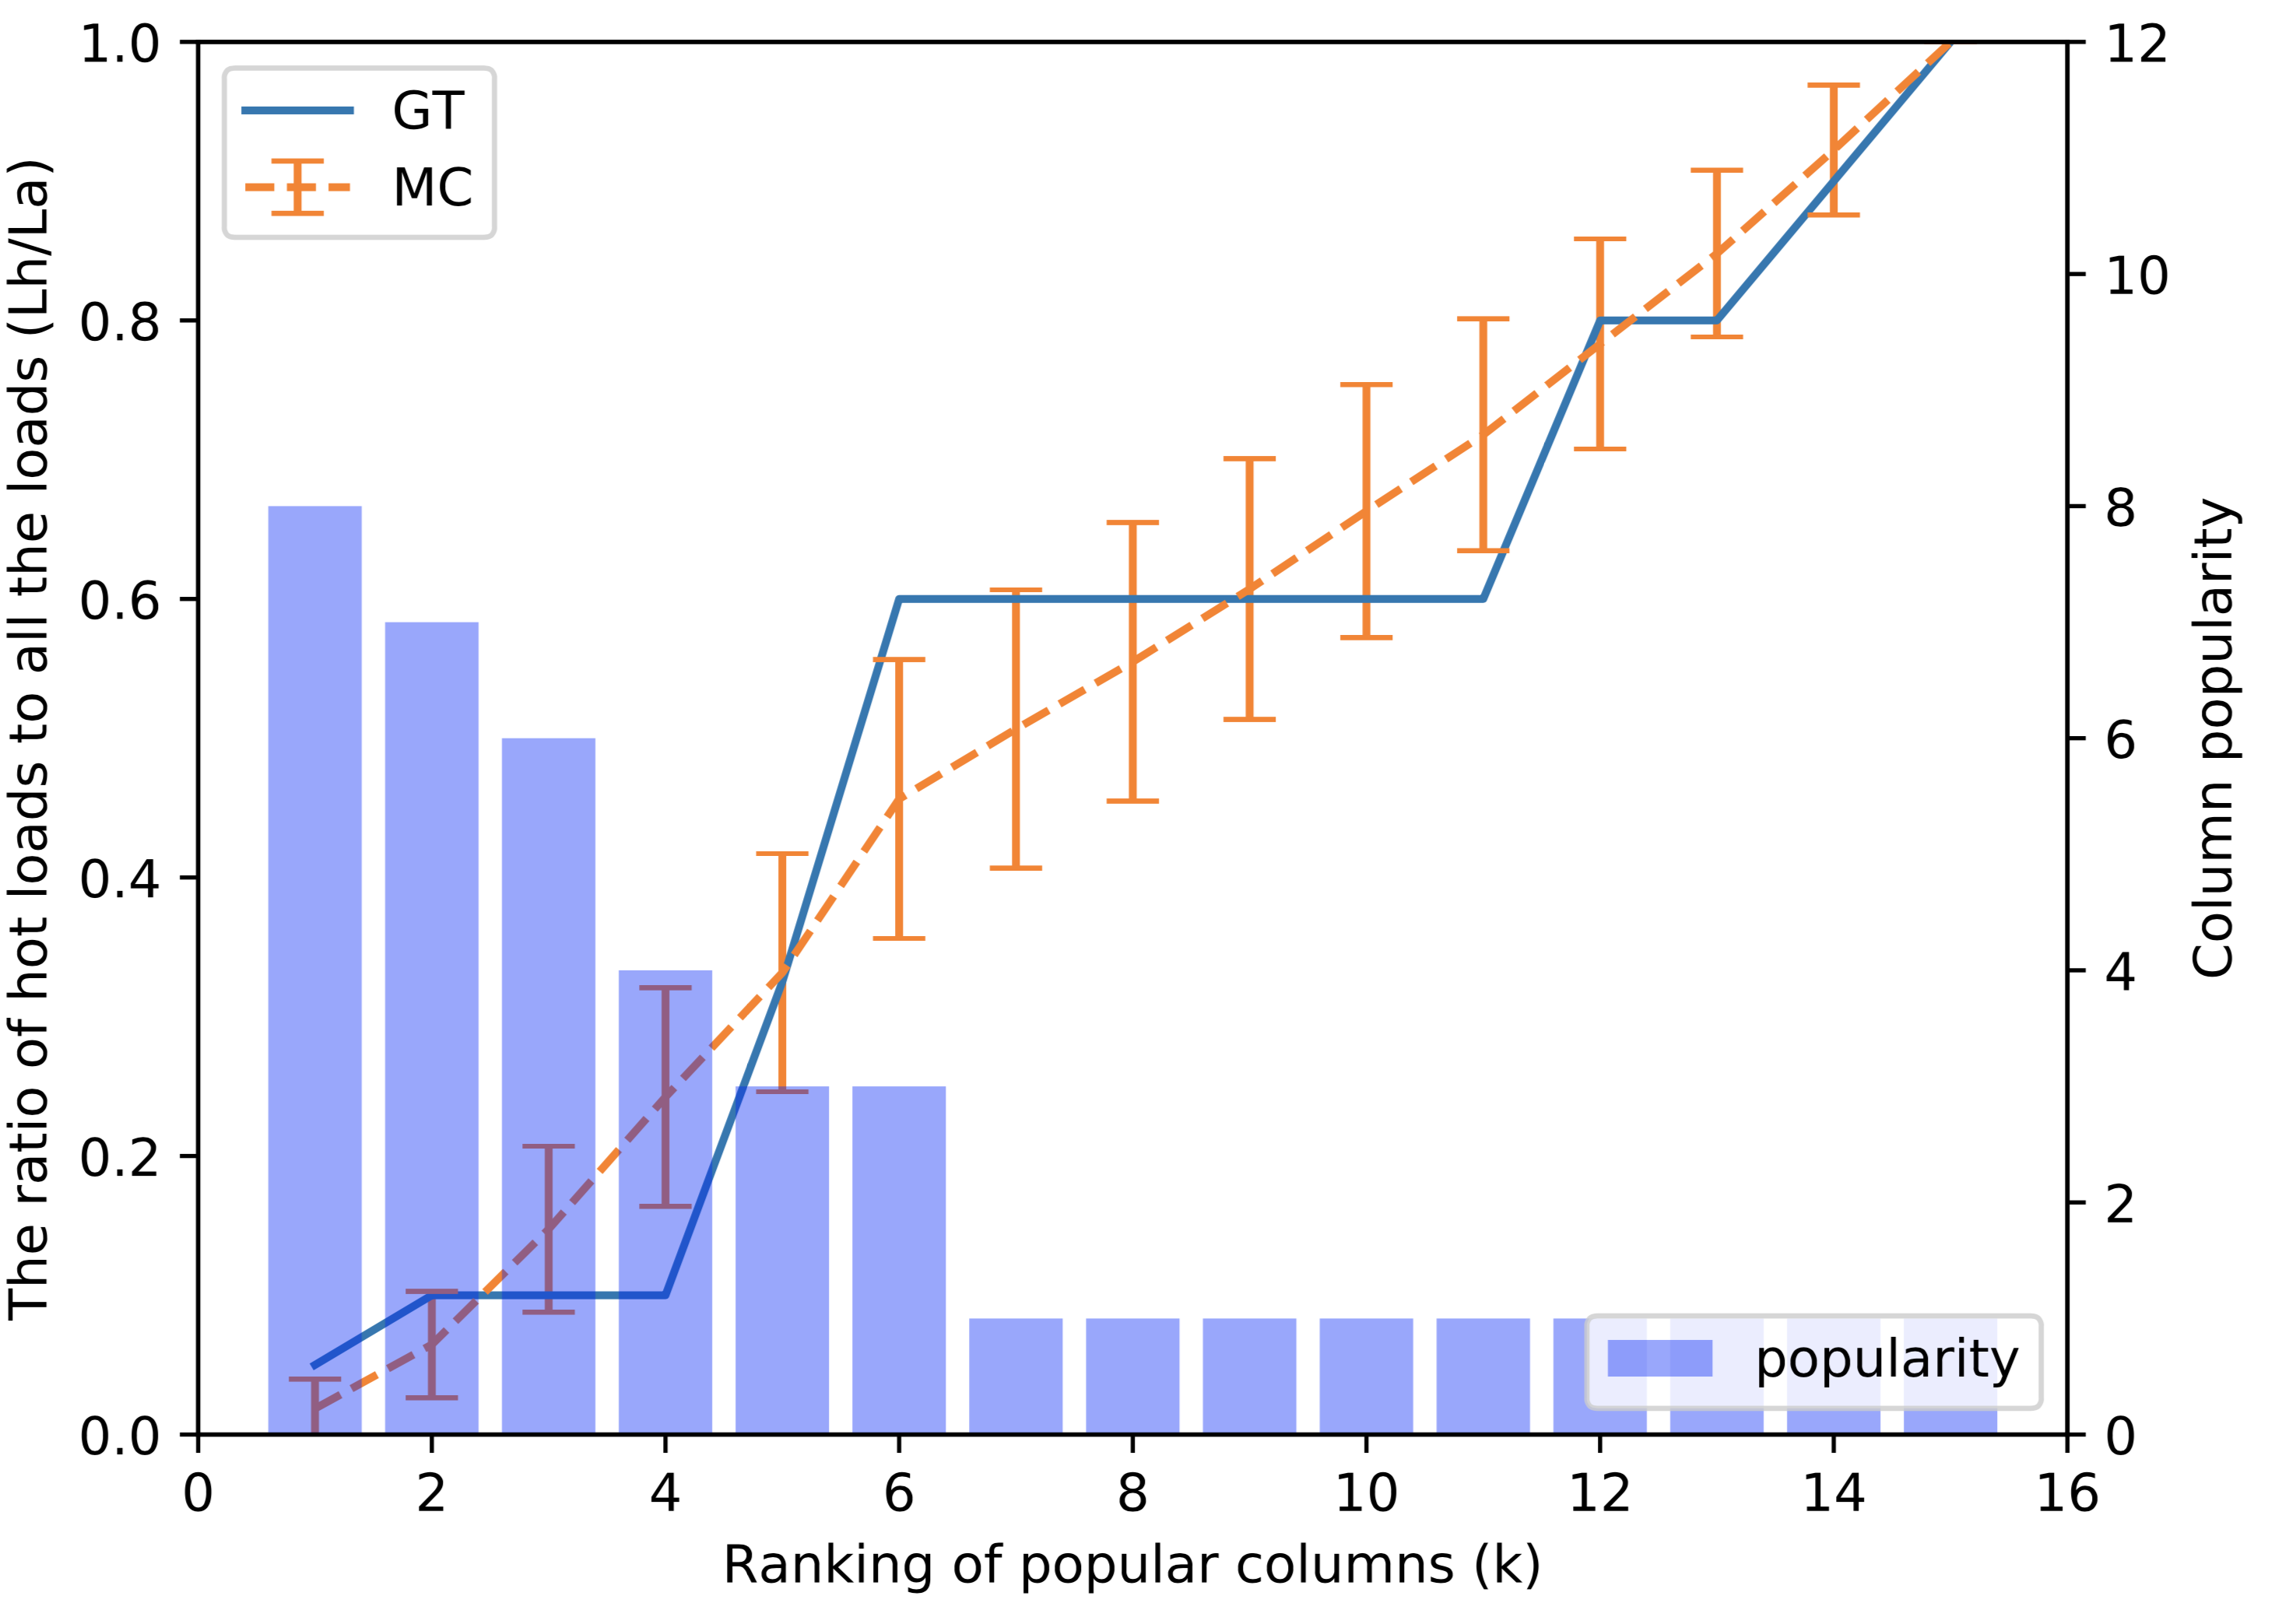
\includegraphics[width=1\textwidth]{img/cw-cache/ca_web_returns}
        \caption{TDC-DS中的 $web\_returns$ 表}
        \label{fig:ca-wr}
    \end{subfigure}%
    
    \begin{subfigure}[t]{0.5\textwidth}
        \centering
        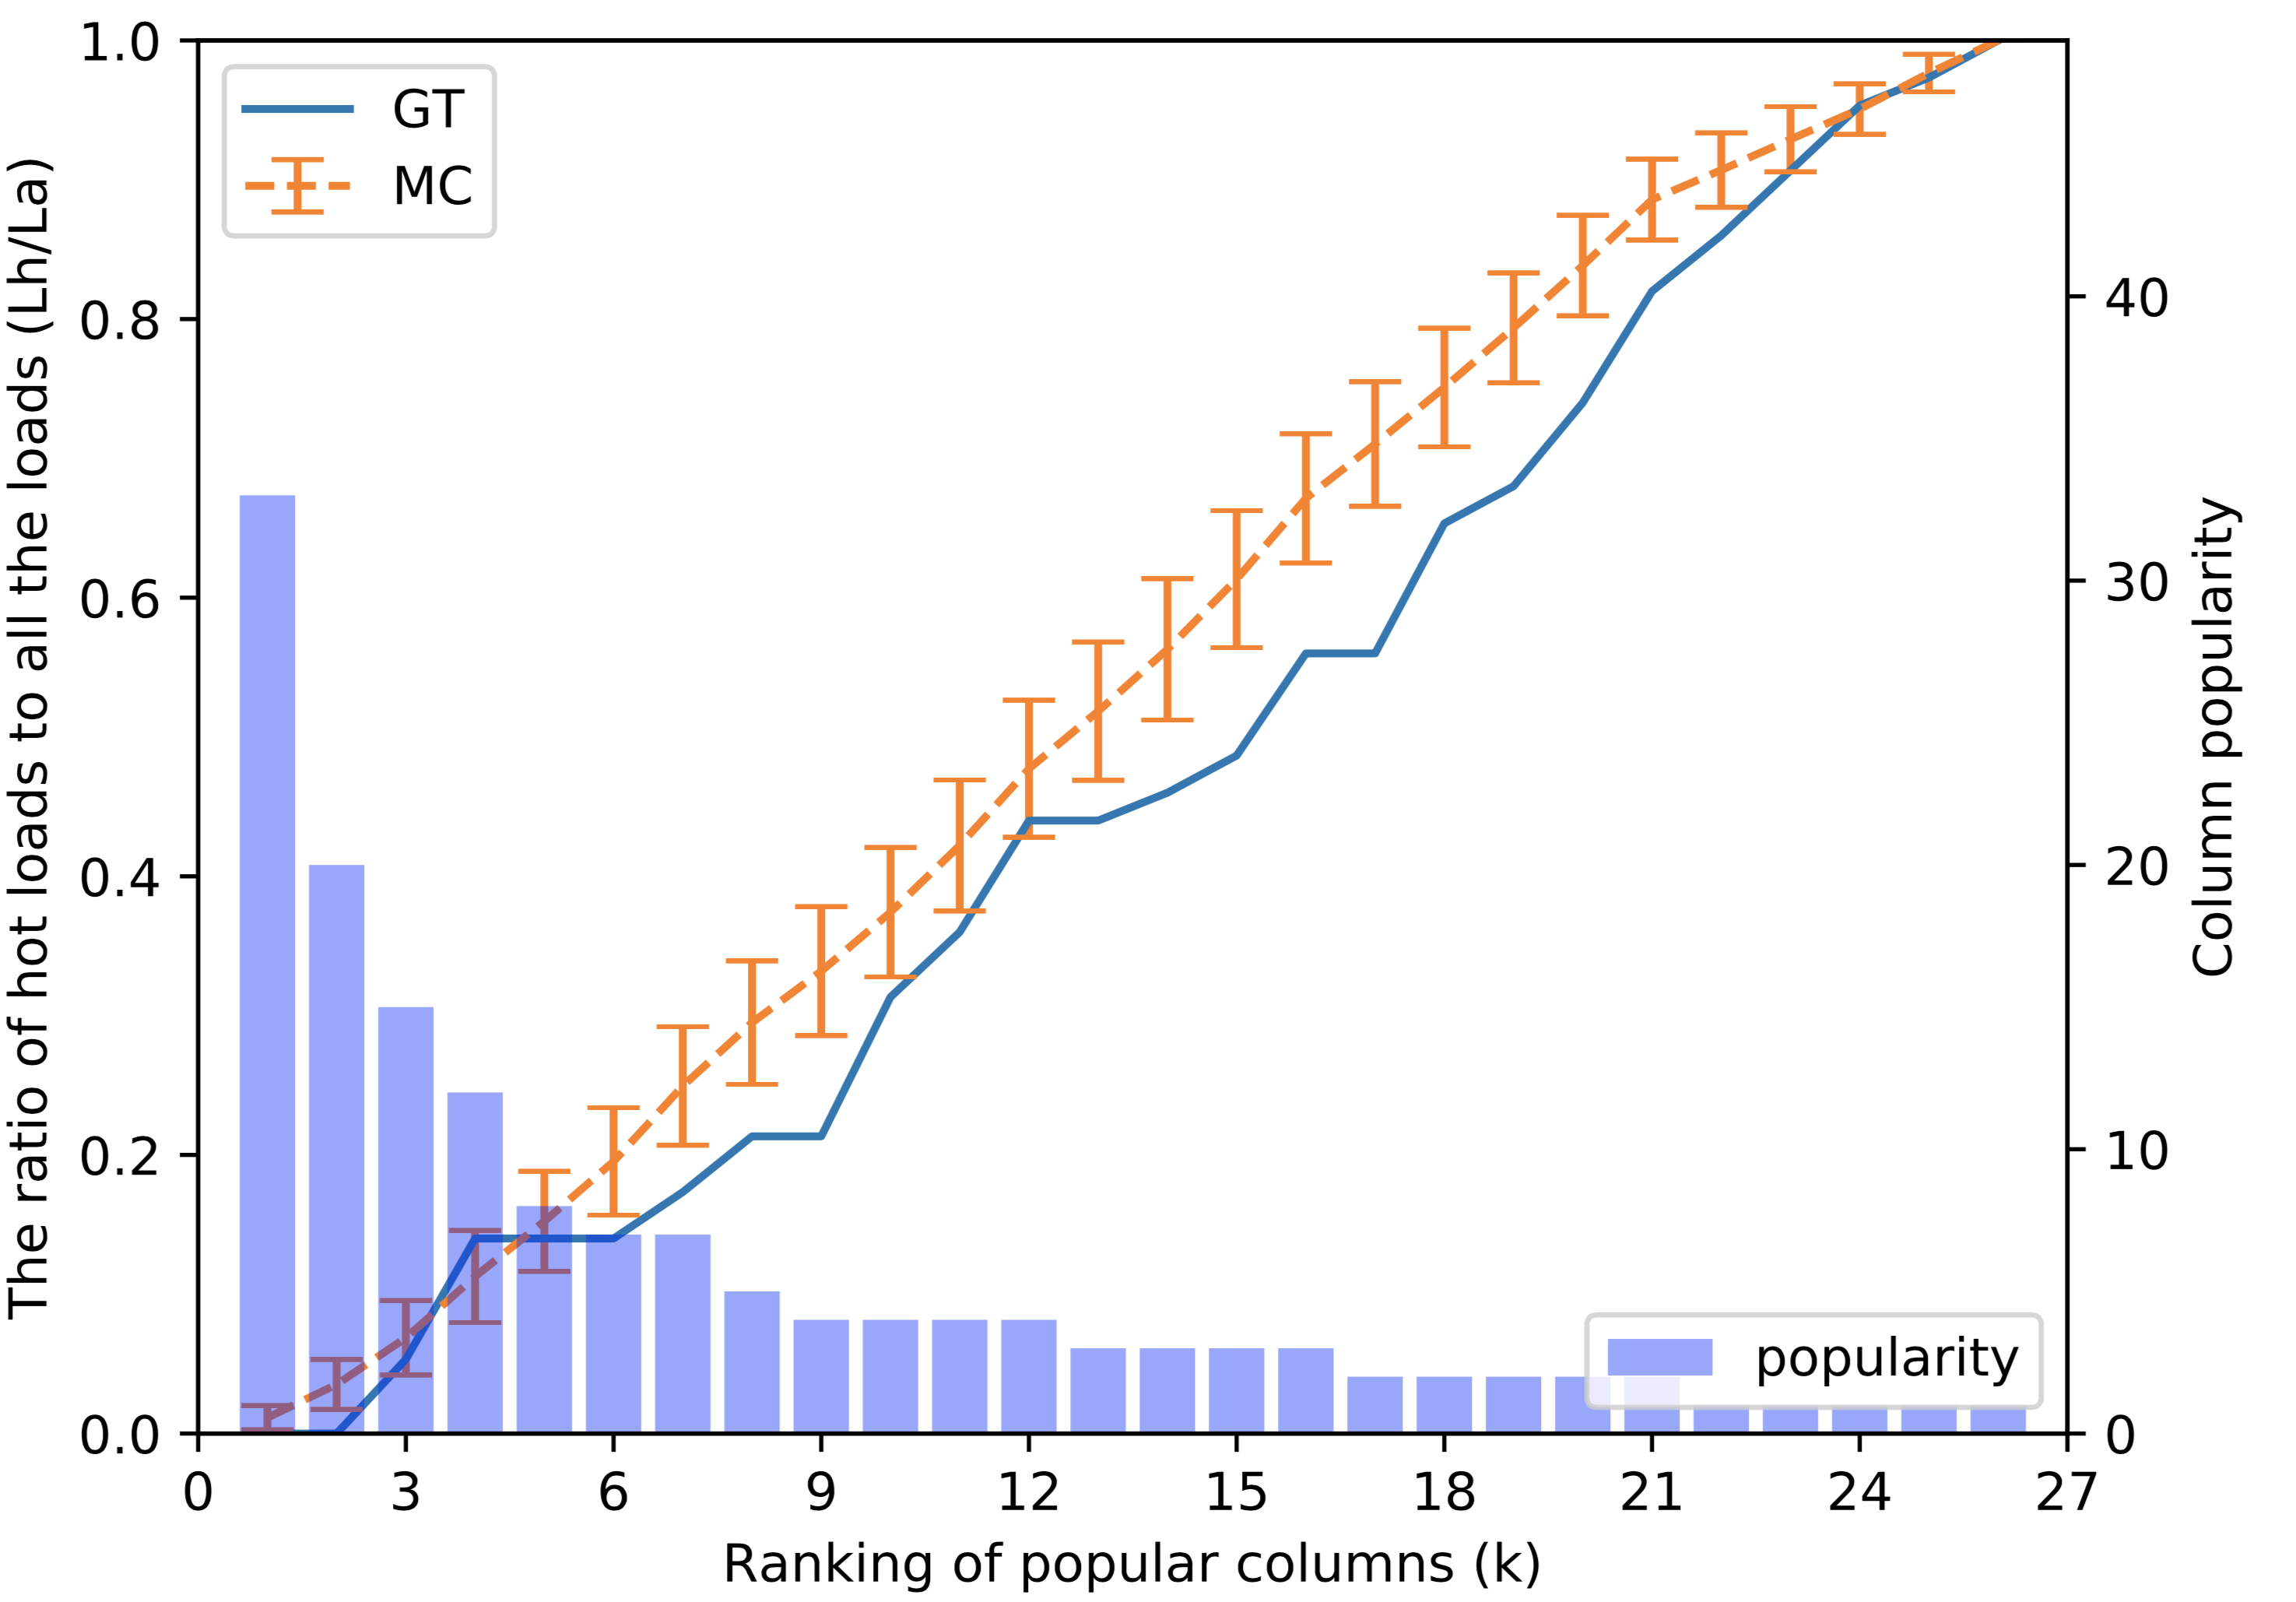
\includegraphics[width=1\textwidth]{img/cw-cache/ca_web_sales}
        \caption{TDC-DS中的 $web\_sales$ t表}
        \label{fig:ca-ws}
    \end{subfigure}%
    \caption{列的热度及归一化的$L_h$ 和 $k$之间的关系。蒙特卡罗方法 vs. 实际情况(Ground Truth)}
    \label{fig:mc_gt}
    %\vspace{-.1in}
\end{figure}

\subsection{分析}

\par 为分析这个方法,我们简单地假设共有$m$个查询任务,每一个有 $B = \left\{\frac{p_{1}}{m}, \frac{p_{2}}{m}, \dots, \frac{p_{n}}{m}\right\}$ 的概率访问 $n$ 个列。我们的目标是给定 $k$,估算 $L_h$。

\par 考虑一个特定的查询任务 $q_i$,给定 $k$ 值,记$X_i$为一个二元随机变量,表示$q_i$涉及 的列能否被前$k$个最热门的列覆盖。我们有:
\begin{equation}
\Pr\left[X_{i}=1\right]=\prod_{i=k+1}^{n}\left(1-\frac{p_{i}}{m}\right)
\end{equation}

\par 假设来自查询任务$q_i$的负载是$d_i$,其中$d_i$是其访问的列的大小之和。如果$X_i =1$,那么$d_i$的期望值为:
\begin{equation}
E\left[d_i\right]=\sum_{i=1}^{k} \frac{p_{i} s_{i}}{m}=\frac{\sum_{i=1}^{k} l_{i}}{m}
\end{equation}

记$X$为可以由前$k$个最热门的列承担的查询任务的数量,则:
\begin{equation}
X = \sum_{i=1}^m X_i = m \prod_{i=k+1}^{n}\left(1-\frac{p_{i}}{m}\right)
\end{equation}

因此,对于$L_h$,我们有:
\begin{equation}
\label{equ:lh}
\begin{split}
L_h &= \frac{\sum_{i=1}^{k} l_{i}}{m}  \cdot m \prod_{i=k+1}^{n}\left(1-\frac{p_{i}}{m}\right) \\
&= \sum_{i=1}^{k} l_{i} \prod_{i=k+1}^{n}\left(1-\frac{p_{i}}{m}\right)
\end{split}
\end{equation}

根据等式~\ref{equ:lh},当各个列的负载差异程度很高(highly skewed)的时候,当$k$值较小时,$L_h$随着$k$的增大迅速增大。

\par \noindent \textbf{测量实验2} \quad 我们做实验对比了用等式~\ref{equ:lh}求得的$L_h$的预测值(PV)和通过蒙特卡罗方法得到的$L_h$的值,结果展示在图~\ref{fig:mc_pv} 中,可以看到,两条曲线表现出相似的趋势。我们注意到这两种方法求出的$L_h$的值有误差,原因是我们假设了生成的查询任务是相互独立的,然而这些生成的查询任务包含的列不能超出各个列的定额,这导致在查询任务生成过程后期产生的那些任务实际是有依赖关系的,具体来说,当列 $c_i$的定额用尽,那么后面生成的查询任务访问列$c_i$的概率是$0$而不是$\frac{p_i}{m}$。在实际操作中,我们需要生成的查询任务的数量超出$m$,以便消耗所有列的定额。

\par 事实上,当生成的查询任务的数量变得很大时,公式预测的$L_h$的值能够接近蒙特卡罗方法得到的值。


\begin{figure}[]
    \centering
    \begin{minipage}[t]{0.5\textwidth}
        \begin{subfigure}[t]{1\textwidth}
            \centering
            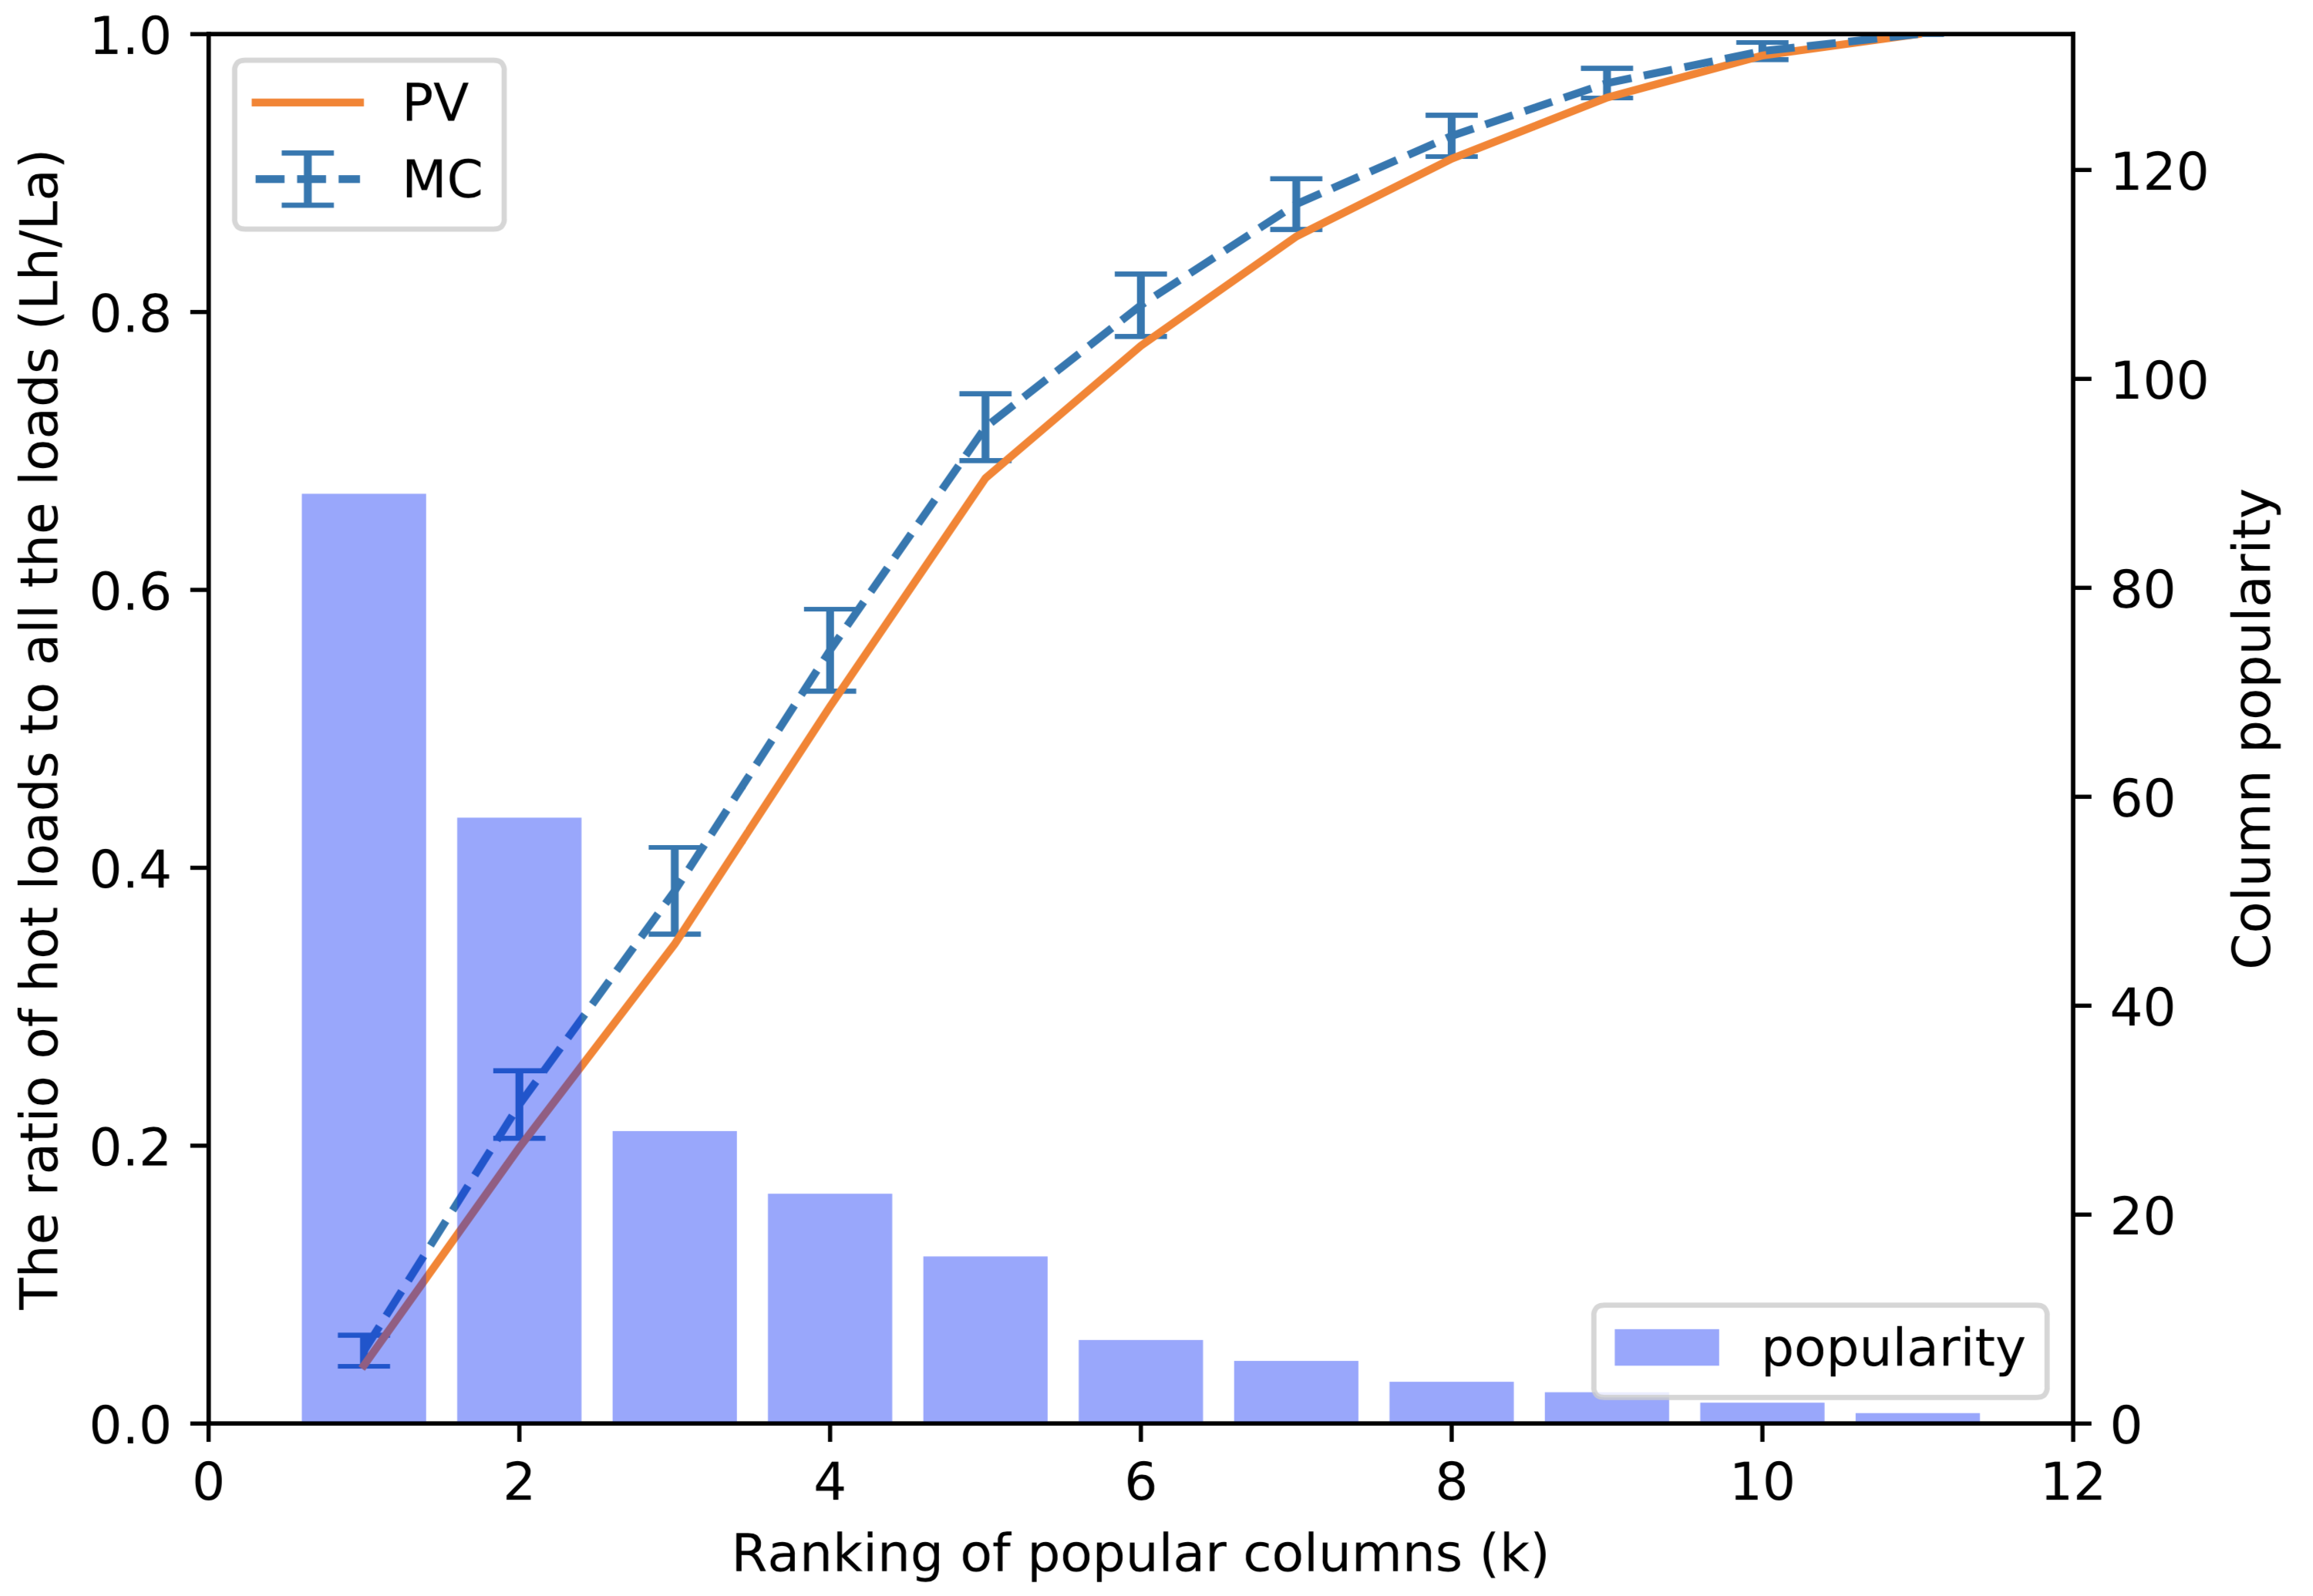
\includegraphics[width=1\textwidth]{img/cw-cache/calc_date_dim}
            \caption{TDC-DS中的 $data\_dim$ 表。}
            \label{fig:calc-dd}
        \end{subfigure}%

        \begin{subfigure}[t]{1\textwidth}
            \centering
            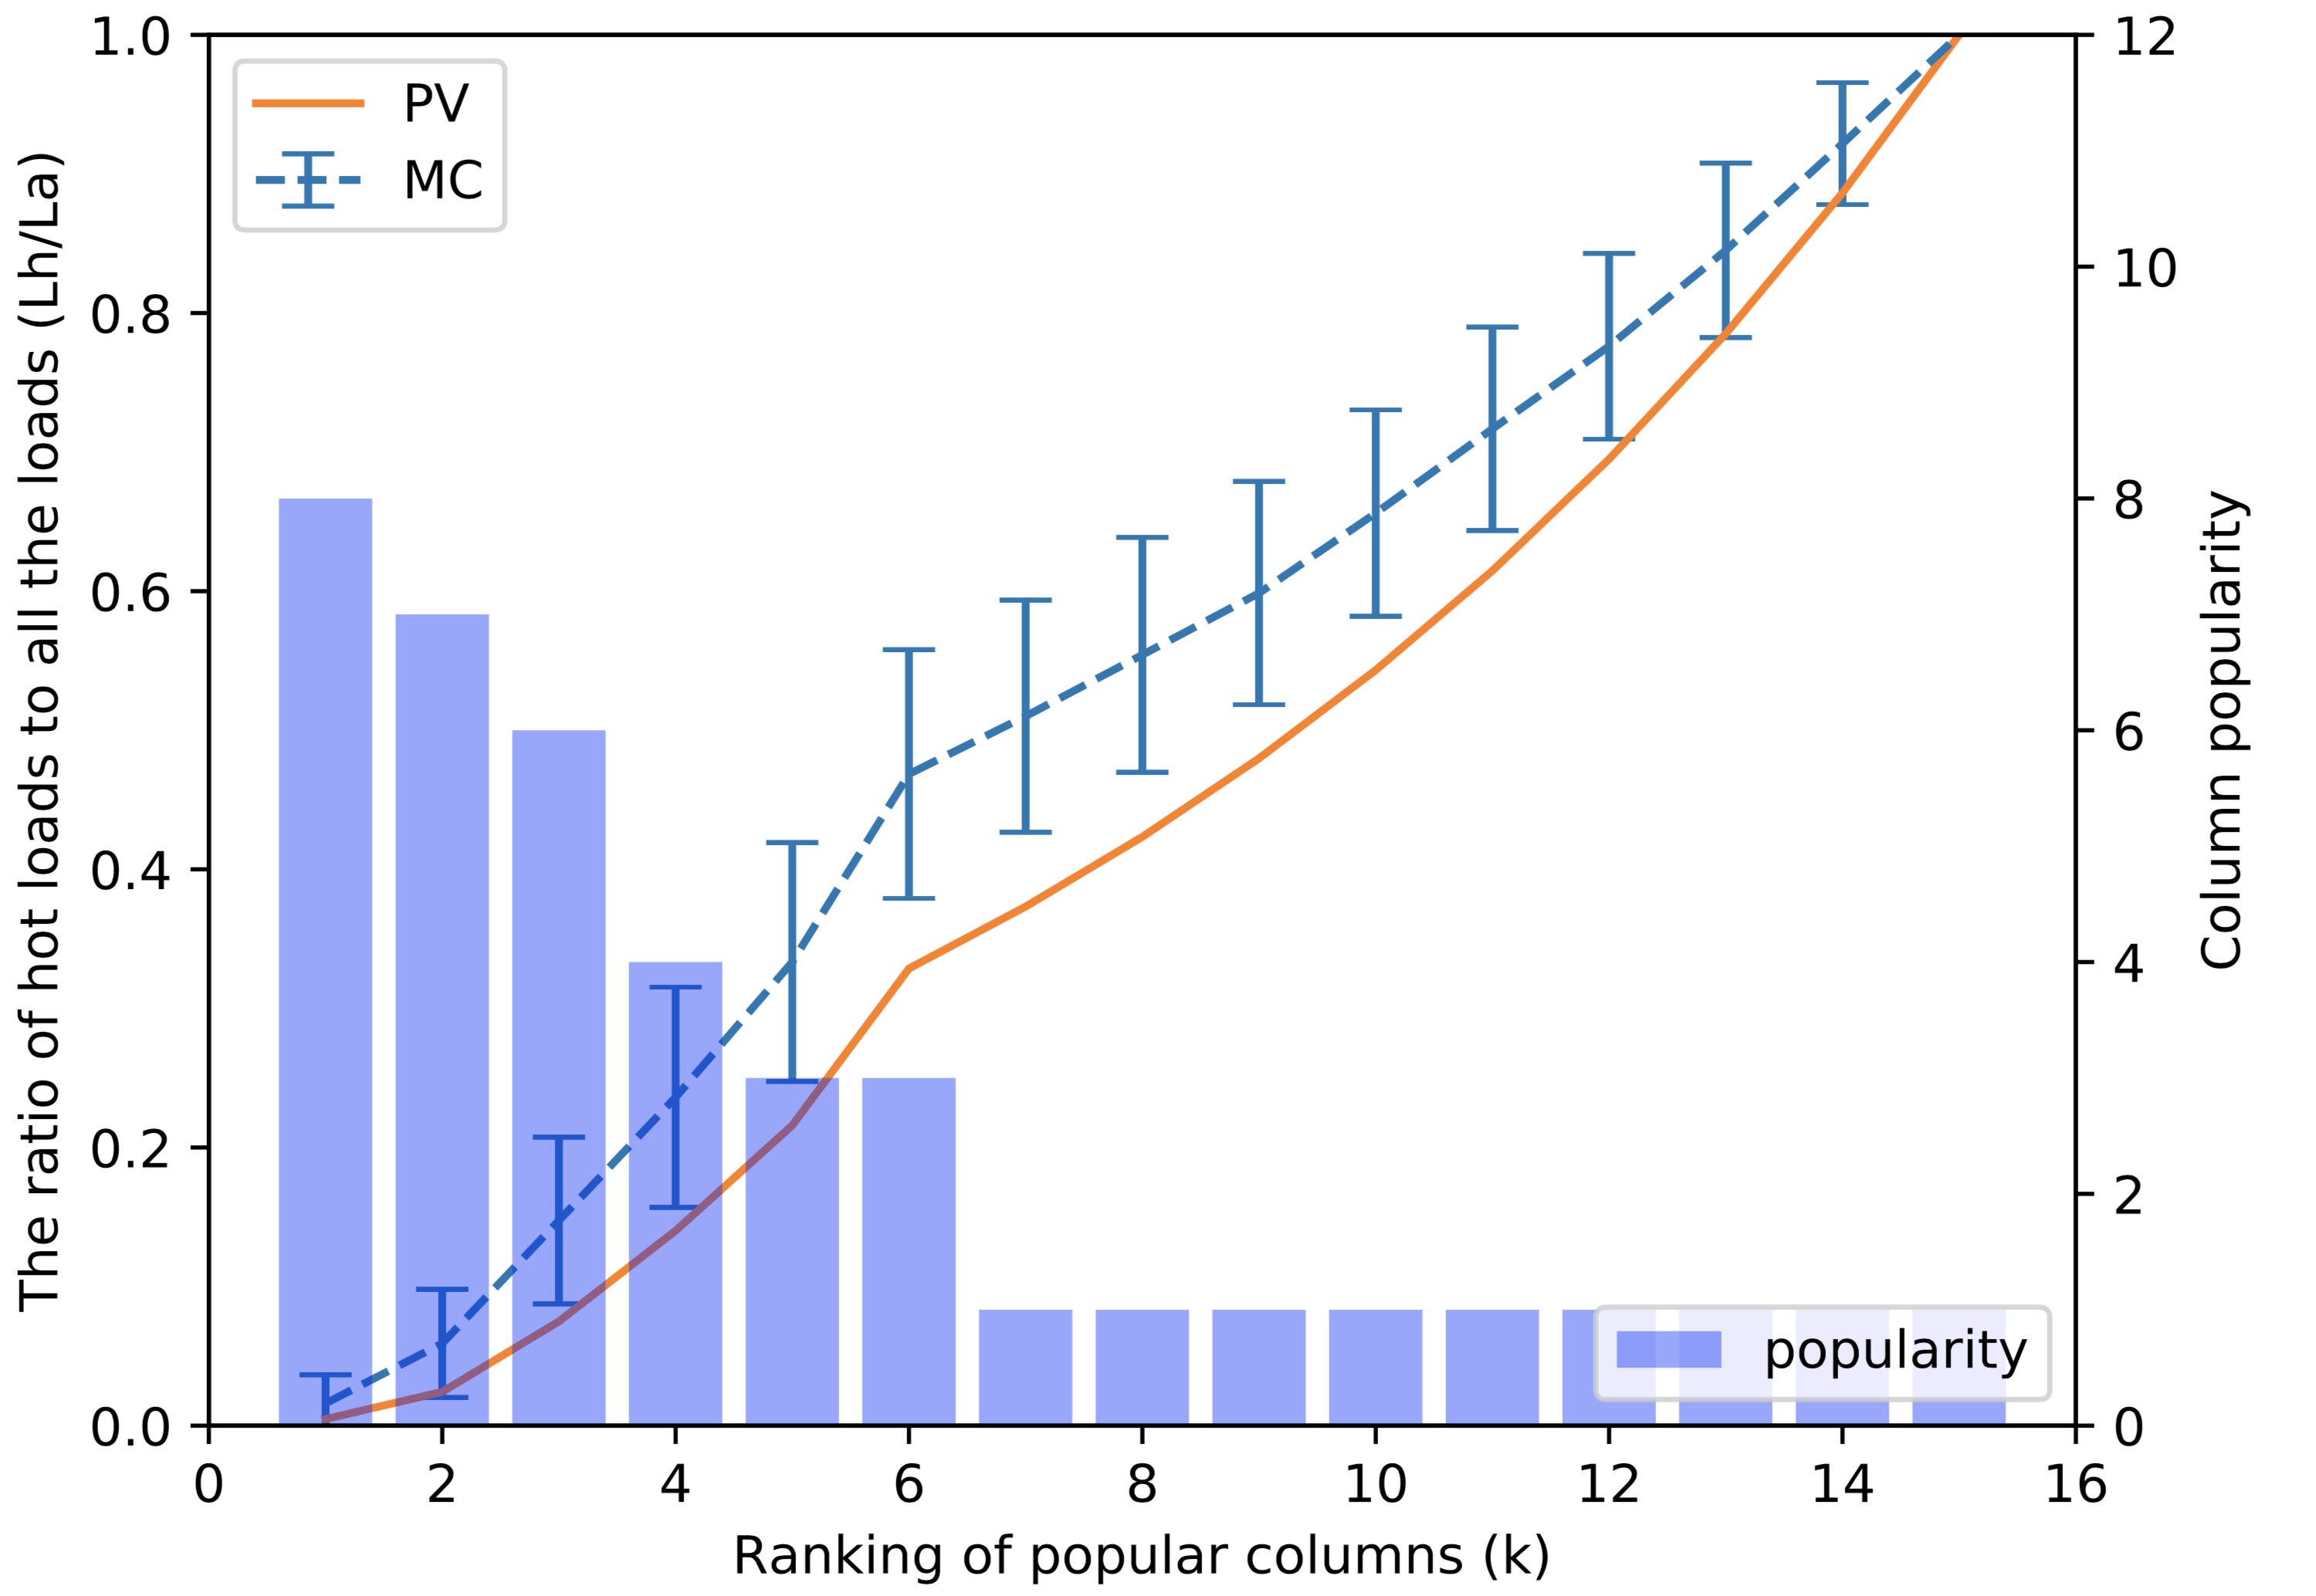
\includegraphics[width=1\textwidth]{img/cw-cache/calc_web_returns}
            \caption{TDC-DS中的 $web\_returns$ t表。}
            \label{fig:calc-wr}
        \end{subfigure}%

        \begin{subfigure}[t]{1\textwidth}
            \centering
            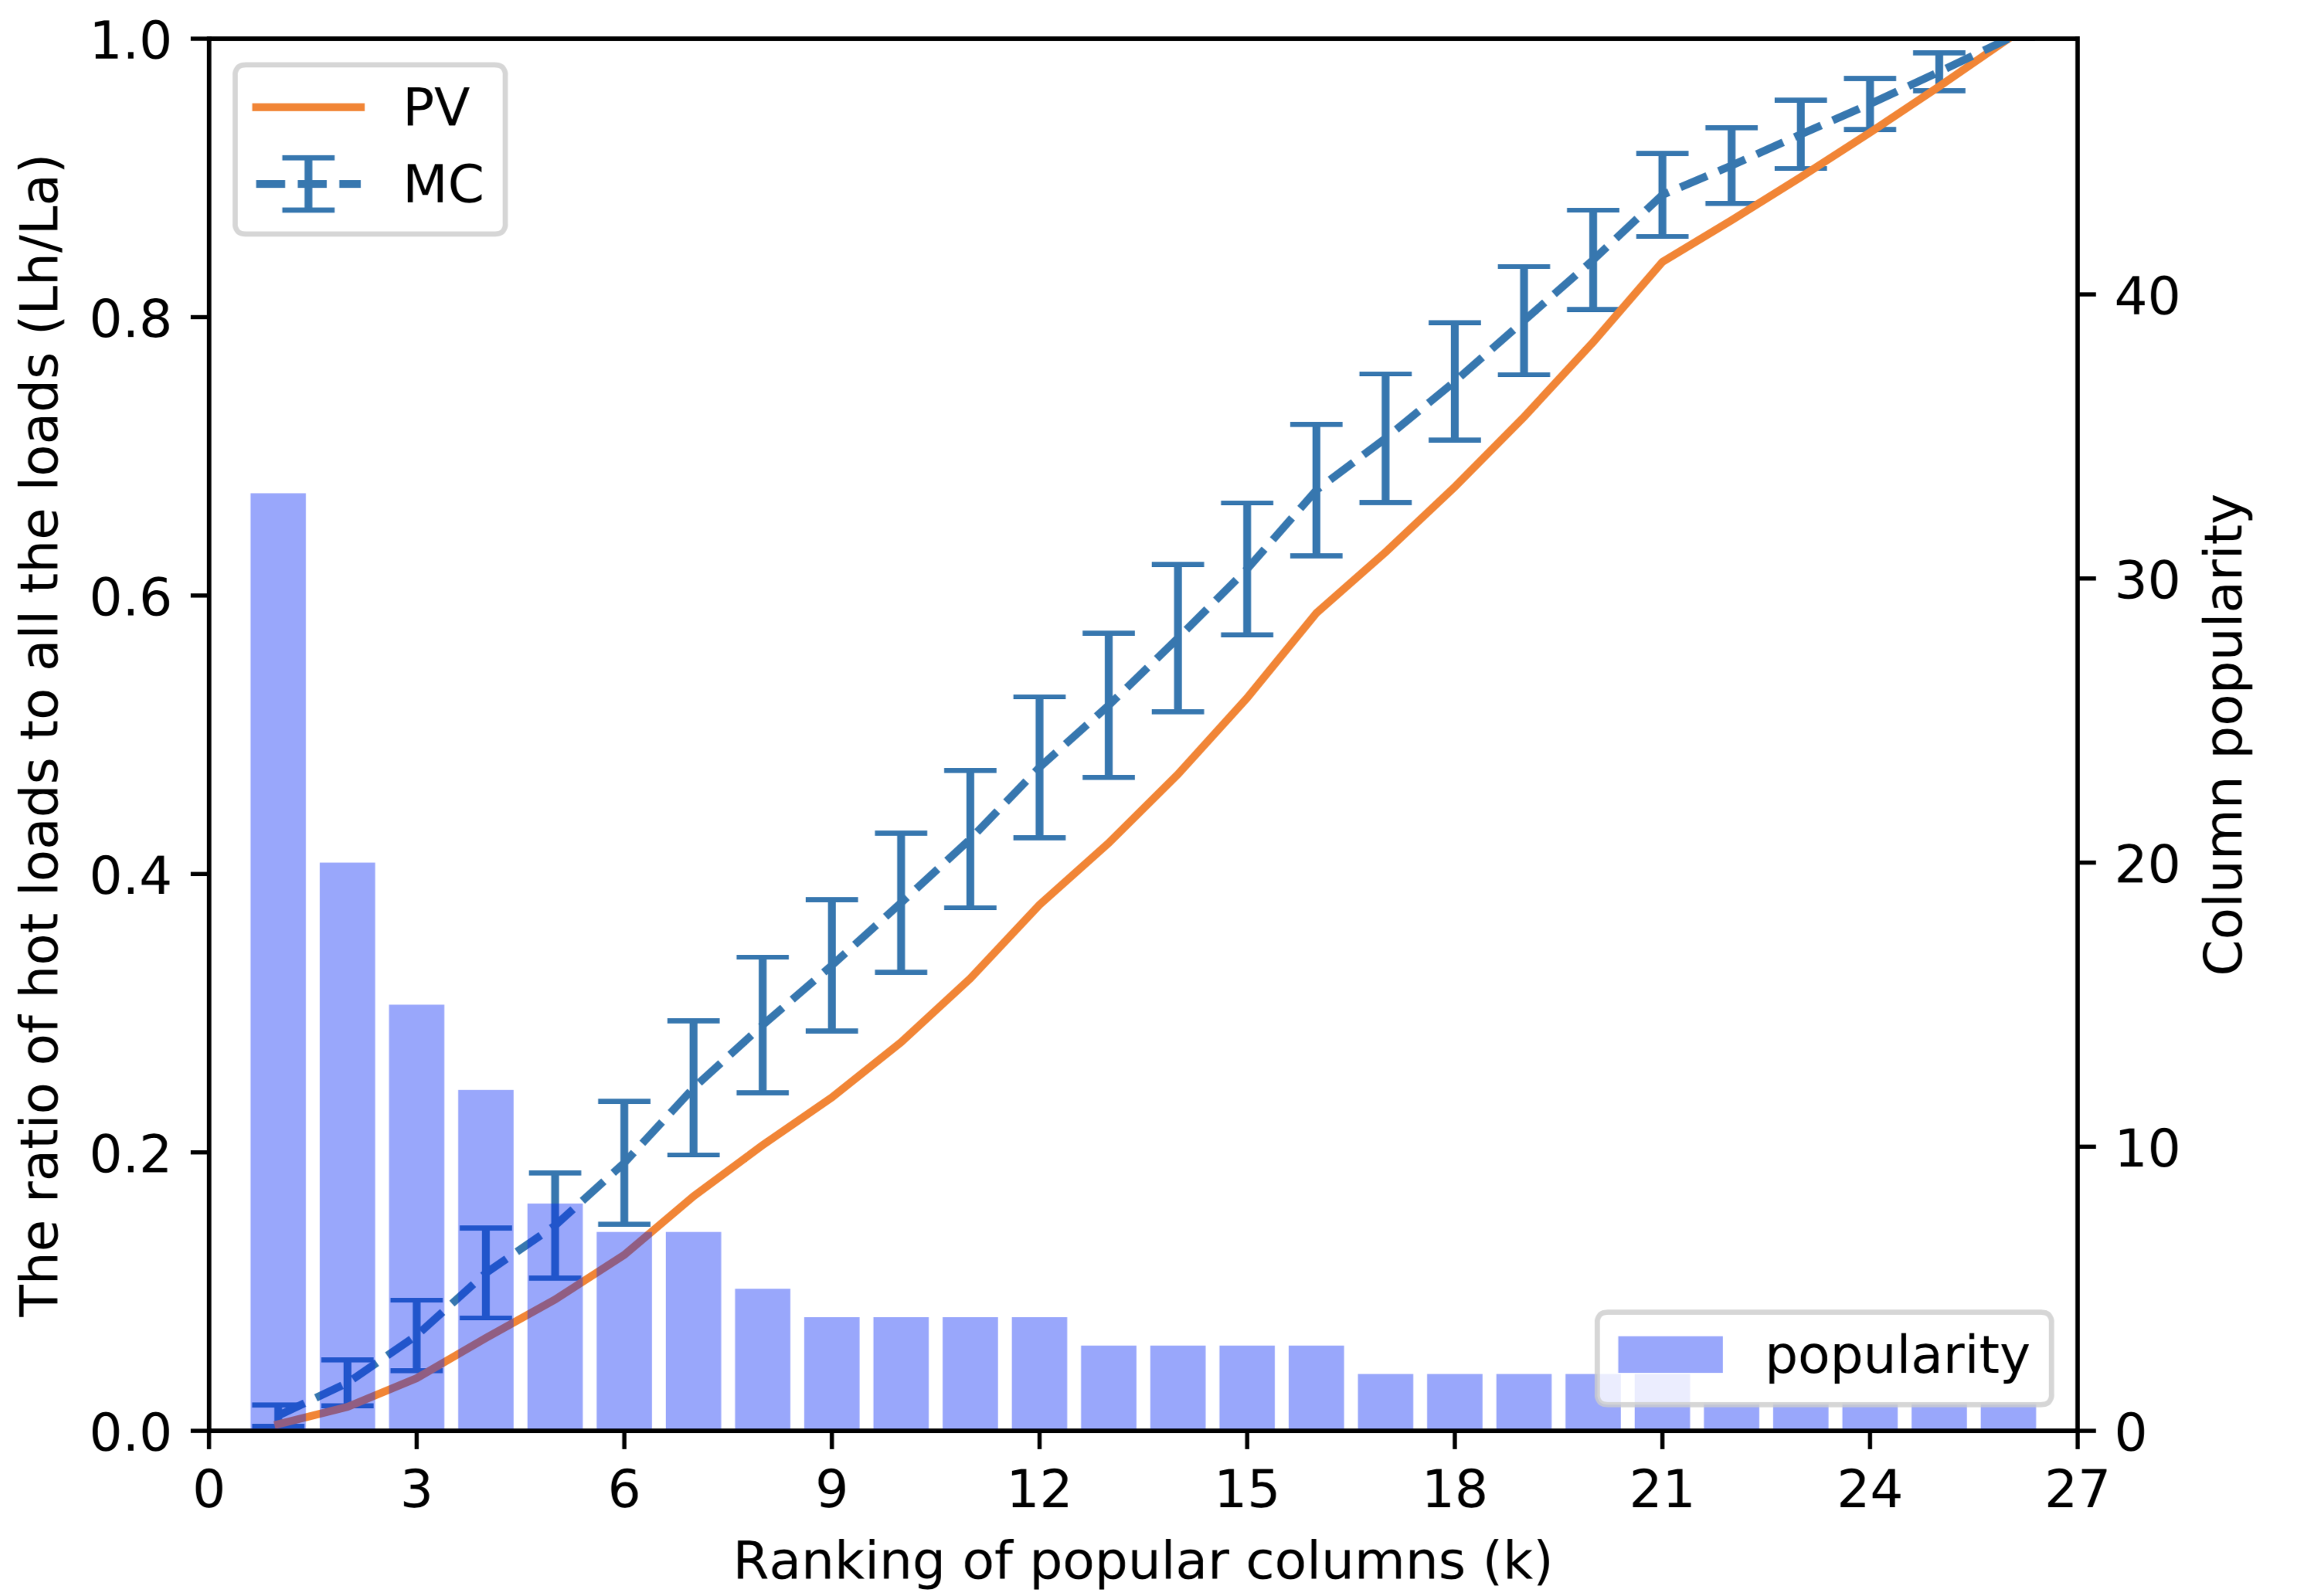
\includegraphics[width=1\textwidth]{img/cw-cache/calc_web_sales}
            \caption{TDC-DS中的 $web\_sales$ 表。}
            \label{fig:calc-ws}
        \end{subfigure}%
        \caption{列的热度及归一化的$L_h$ 和 $k$之间的关系。蒙特卡罗方法 vs. 公式预测}
	    \label{fig:mc_pv}
	    %\vspace{-.1in}
    \end{minipage}%
	\begin{minipage}[t]{0.5\textwidth}
        \centering
        \begin{subfigure}[t]{1\textwidth}
            \centering
            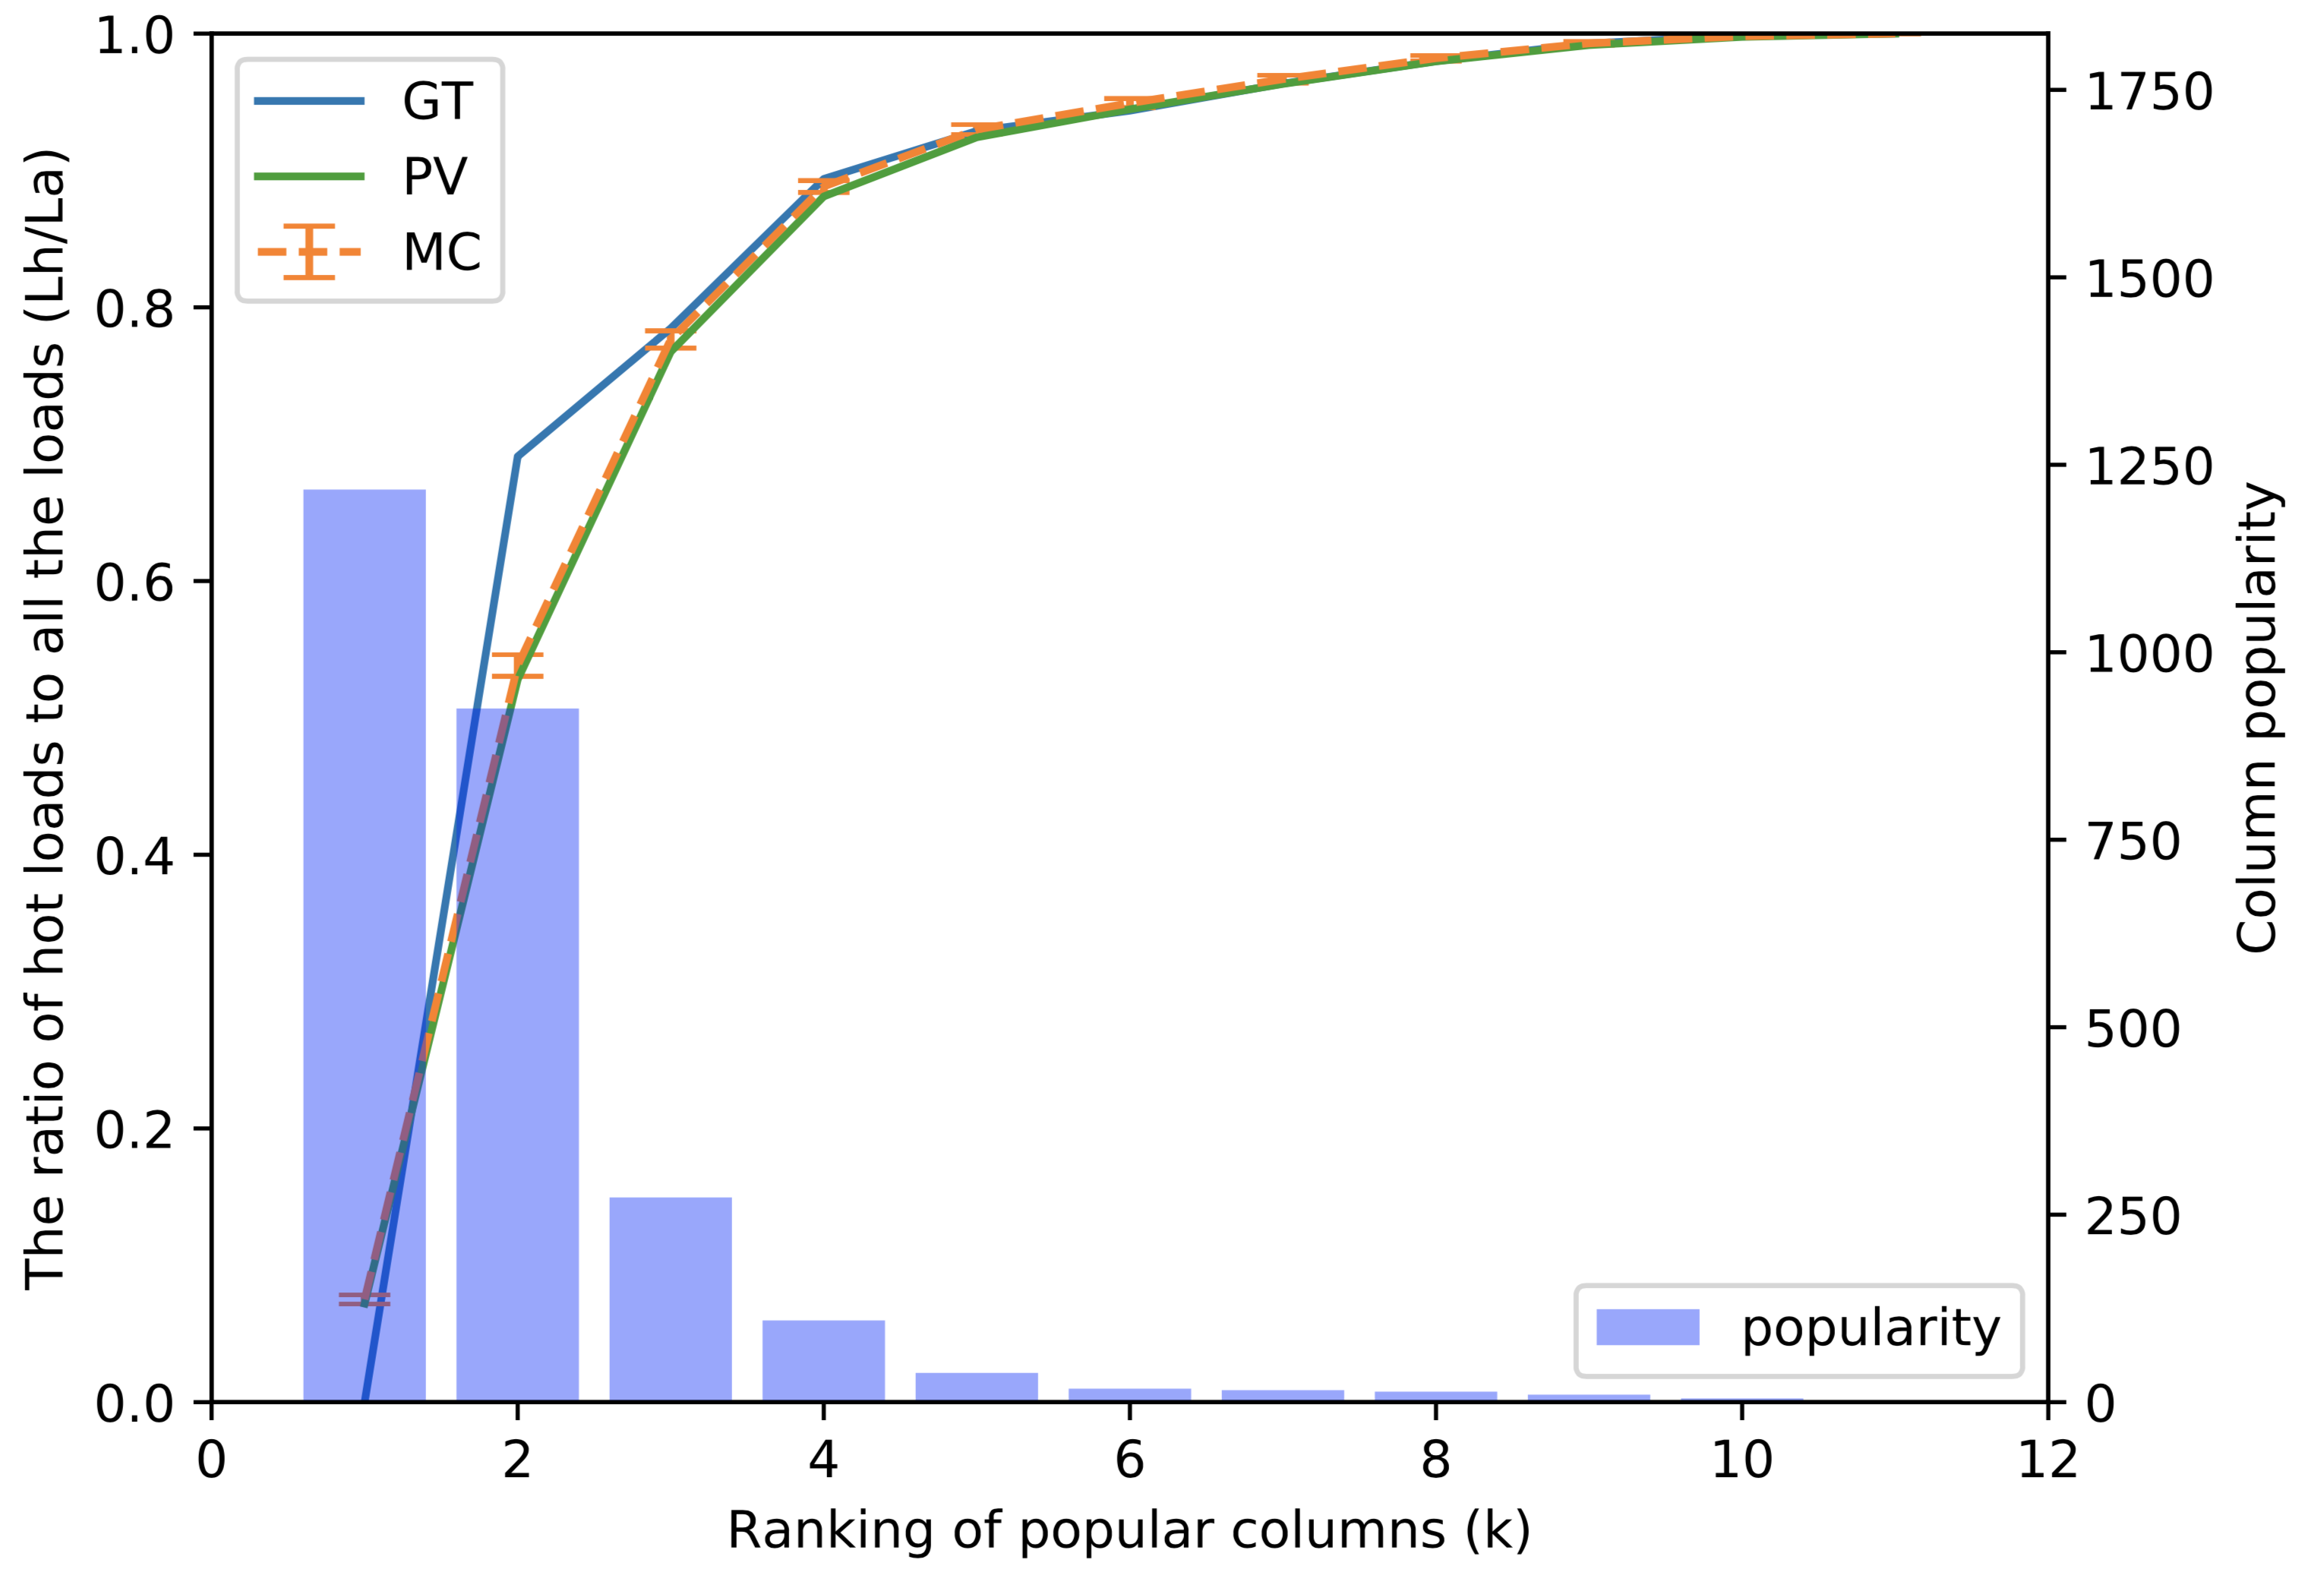
\includegraphics[width=1\textwidth]{img/cw-cache/emul_date_dim}
            \caption{TPC-DS中 $data\_dim$ 表。}
            \label{fig:emul-dd}
        \end{subfigure}%
        
        \begin{subfigure}[t]{1\textwidth}
            \centering
            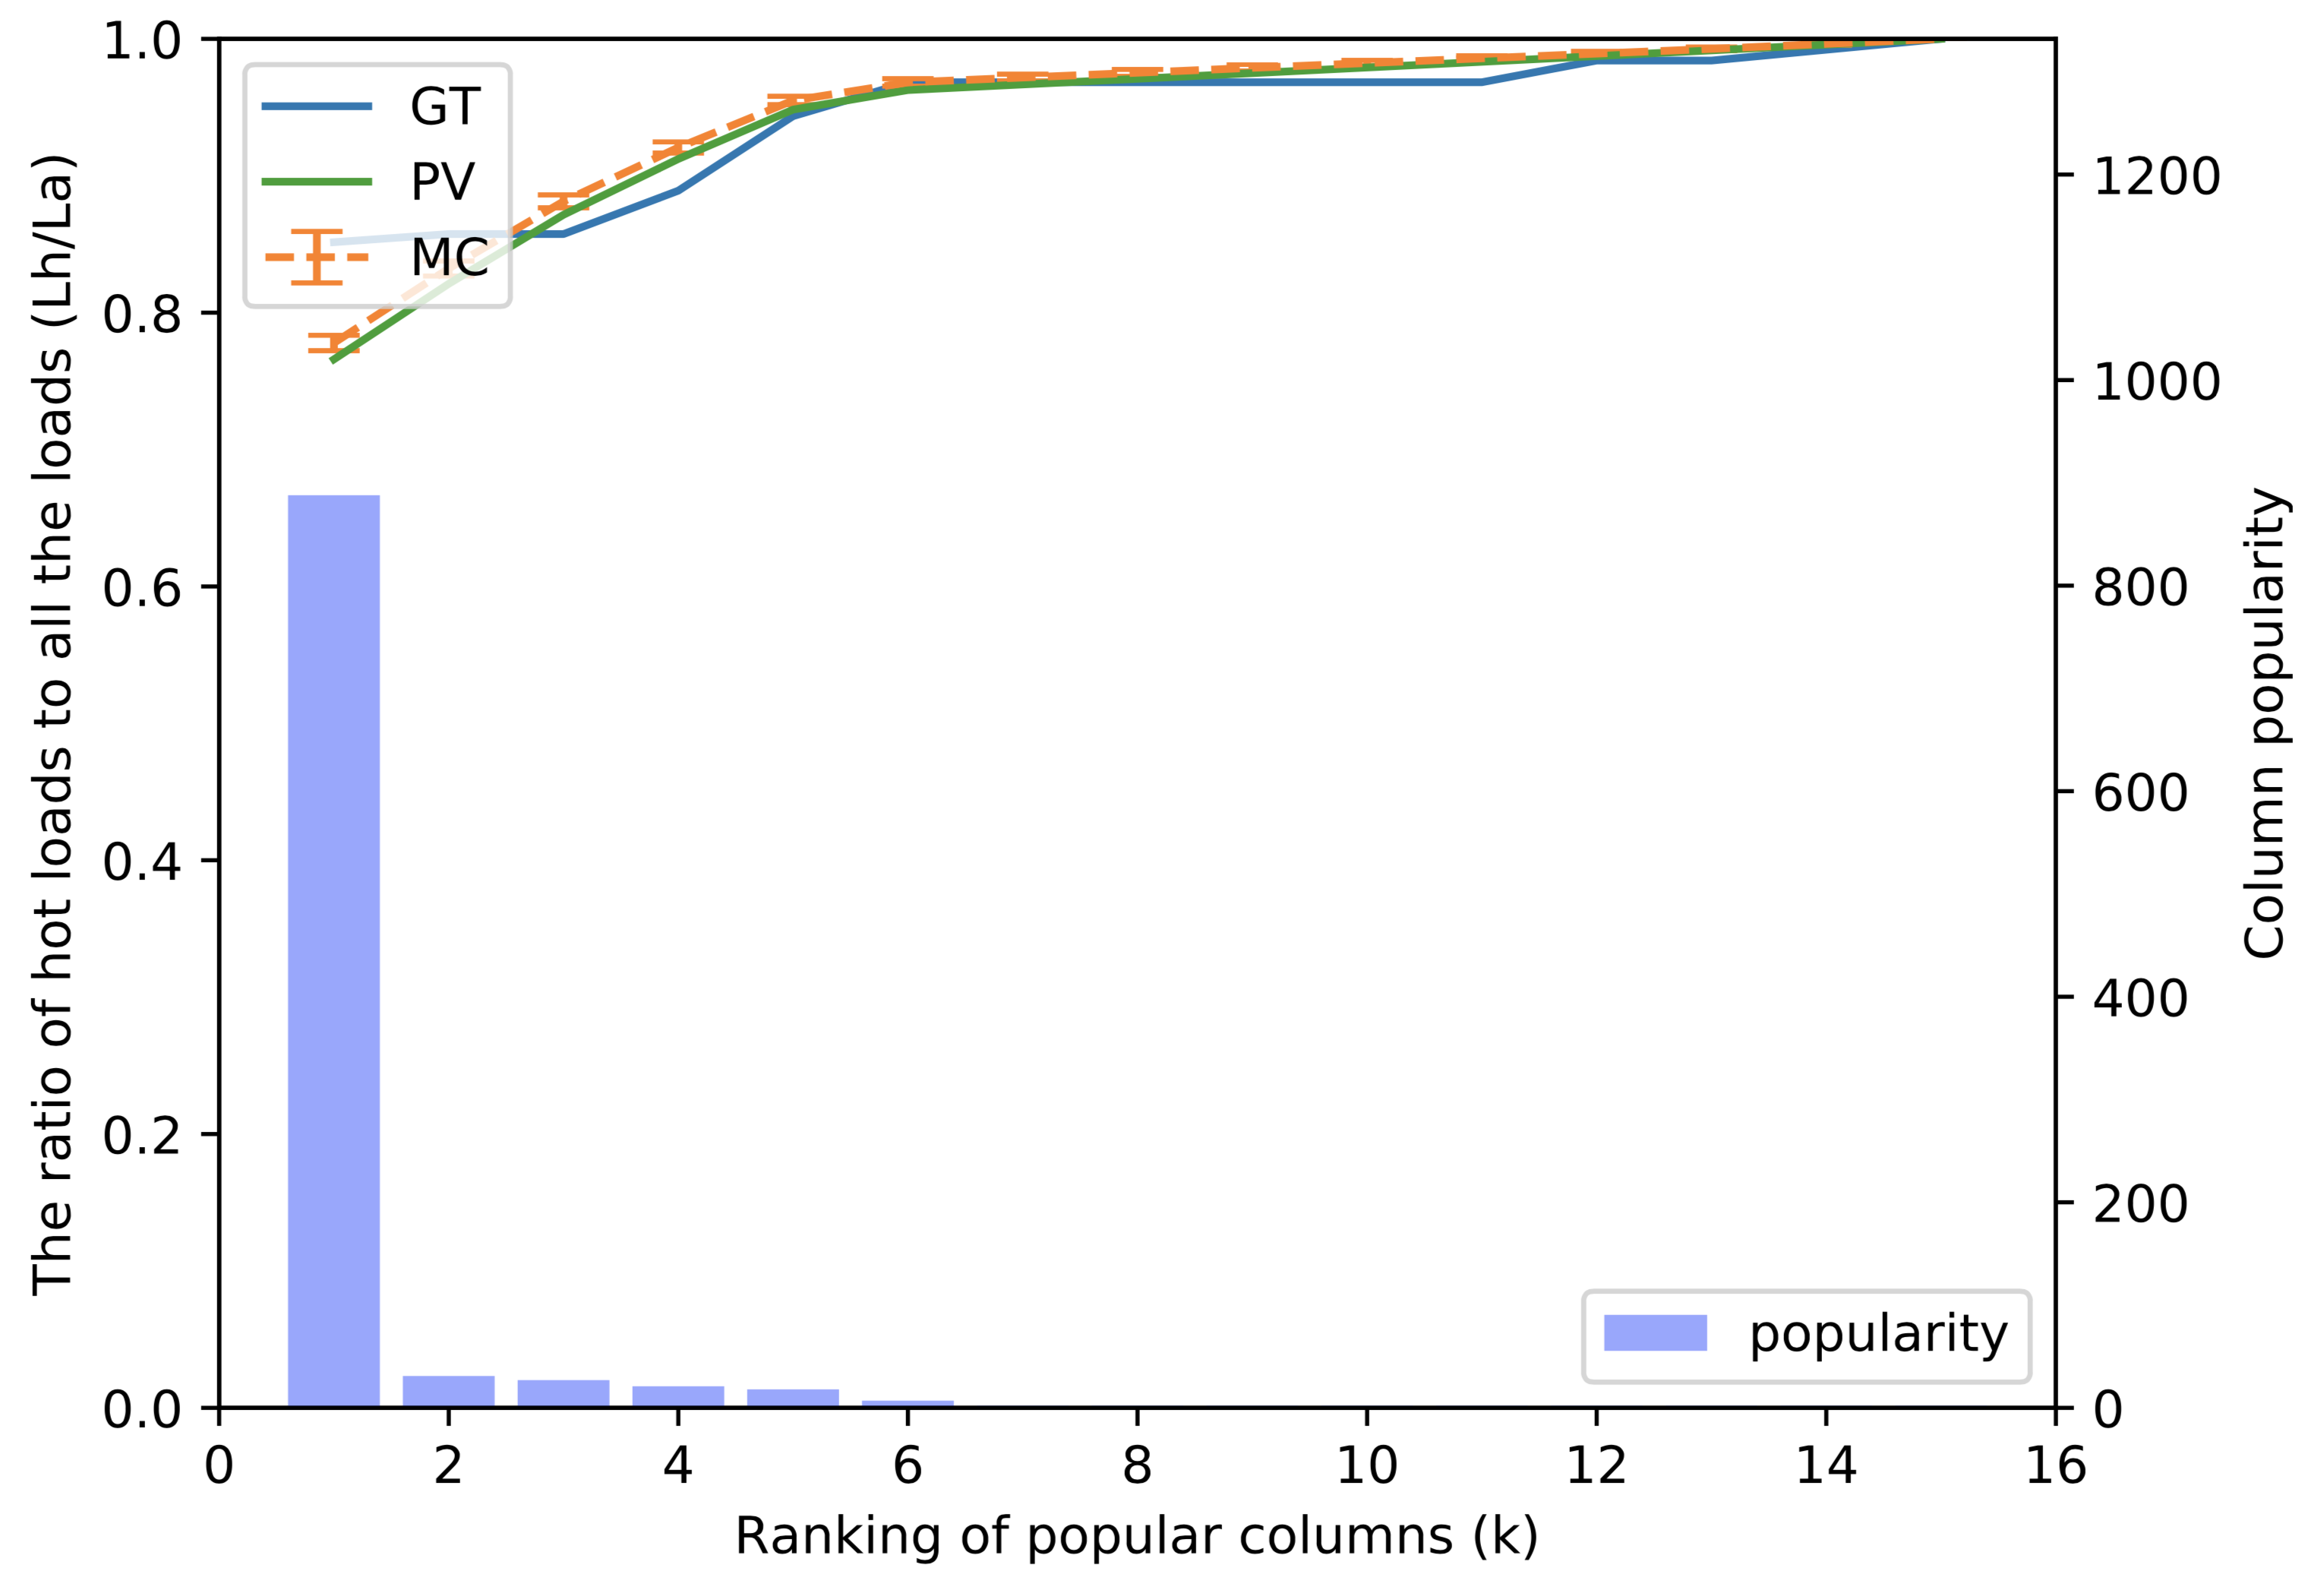
\includegraphics[width=1\textwidth]{img/cw-cache/emul_web_returns}
            \caption{TPC-DS中的 $web\_returns$ 表。}
            \label{fig:emul-wr}
        \end{subfigure}%
        
        \begin{subfigure}[t]{1\textwidth}
            \centering
            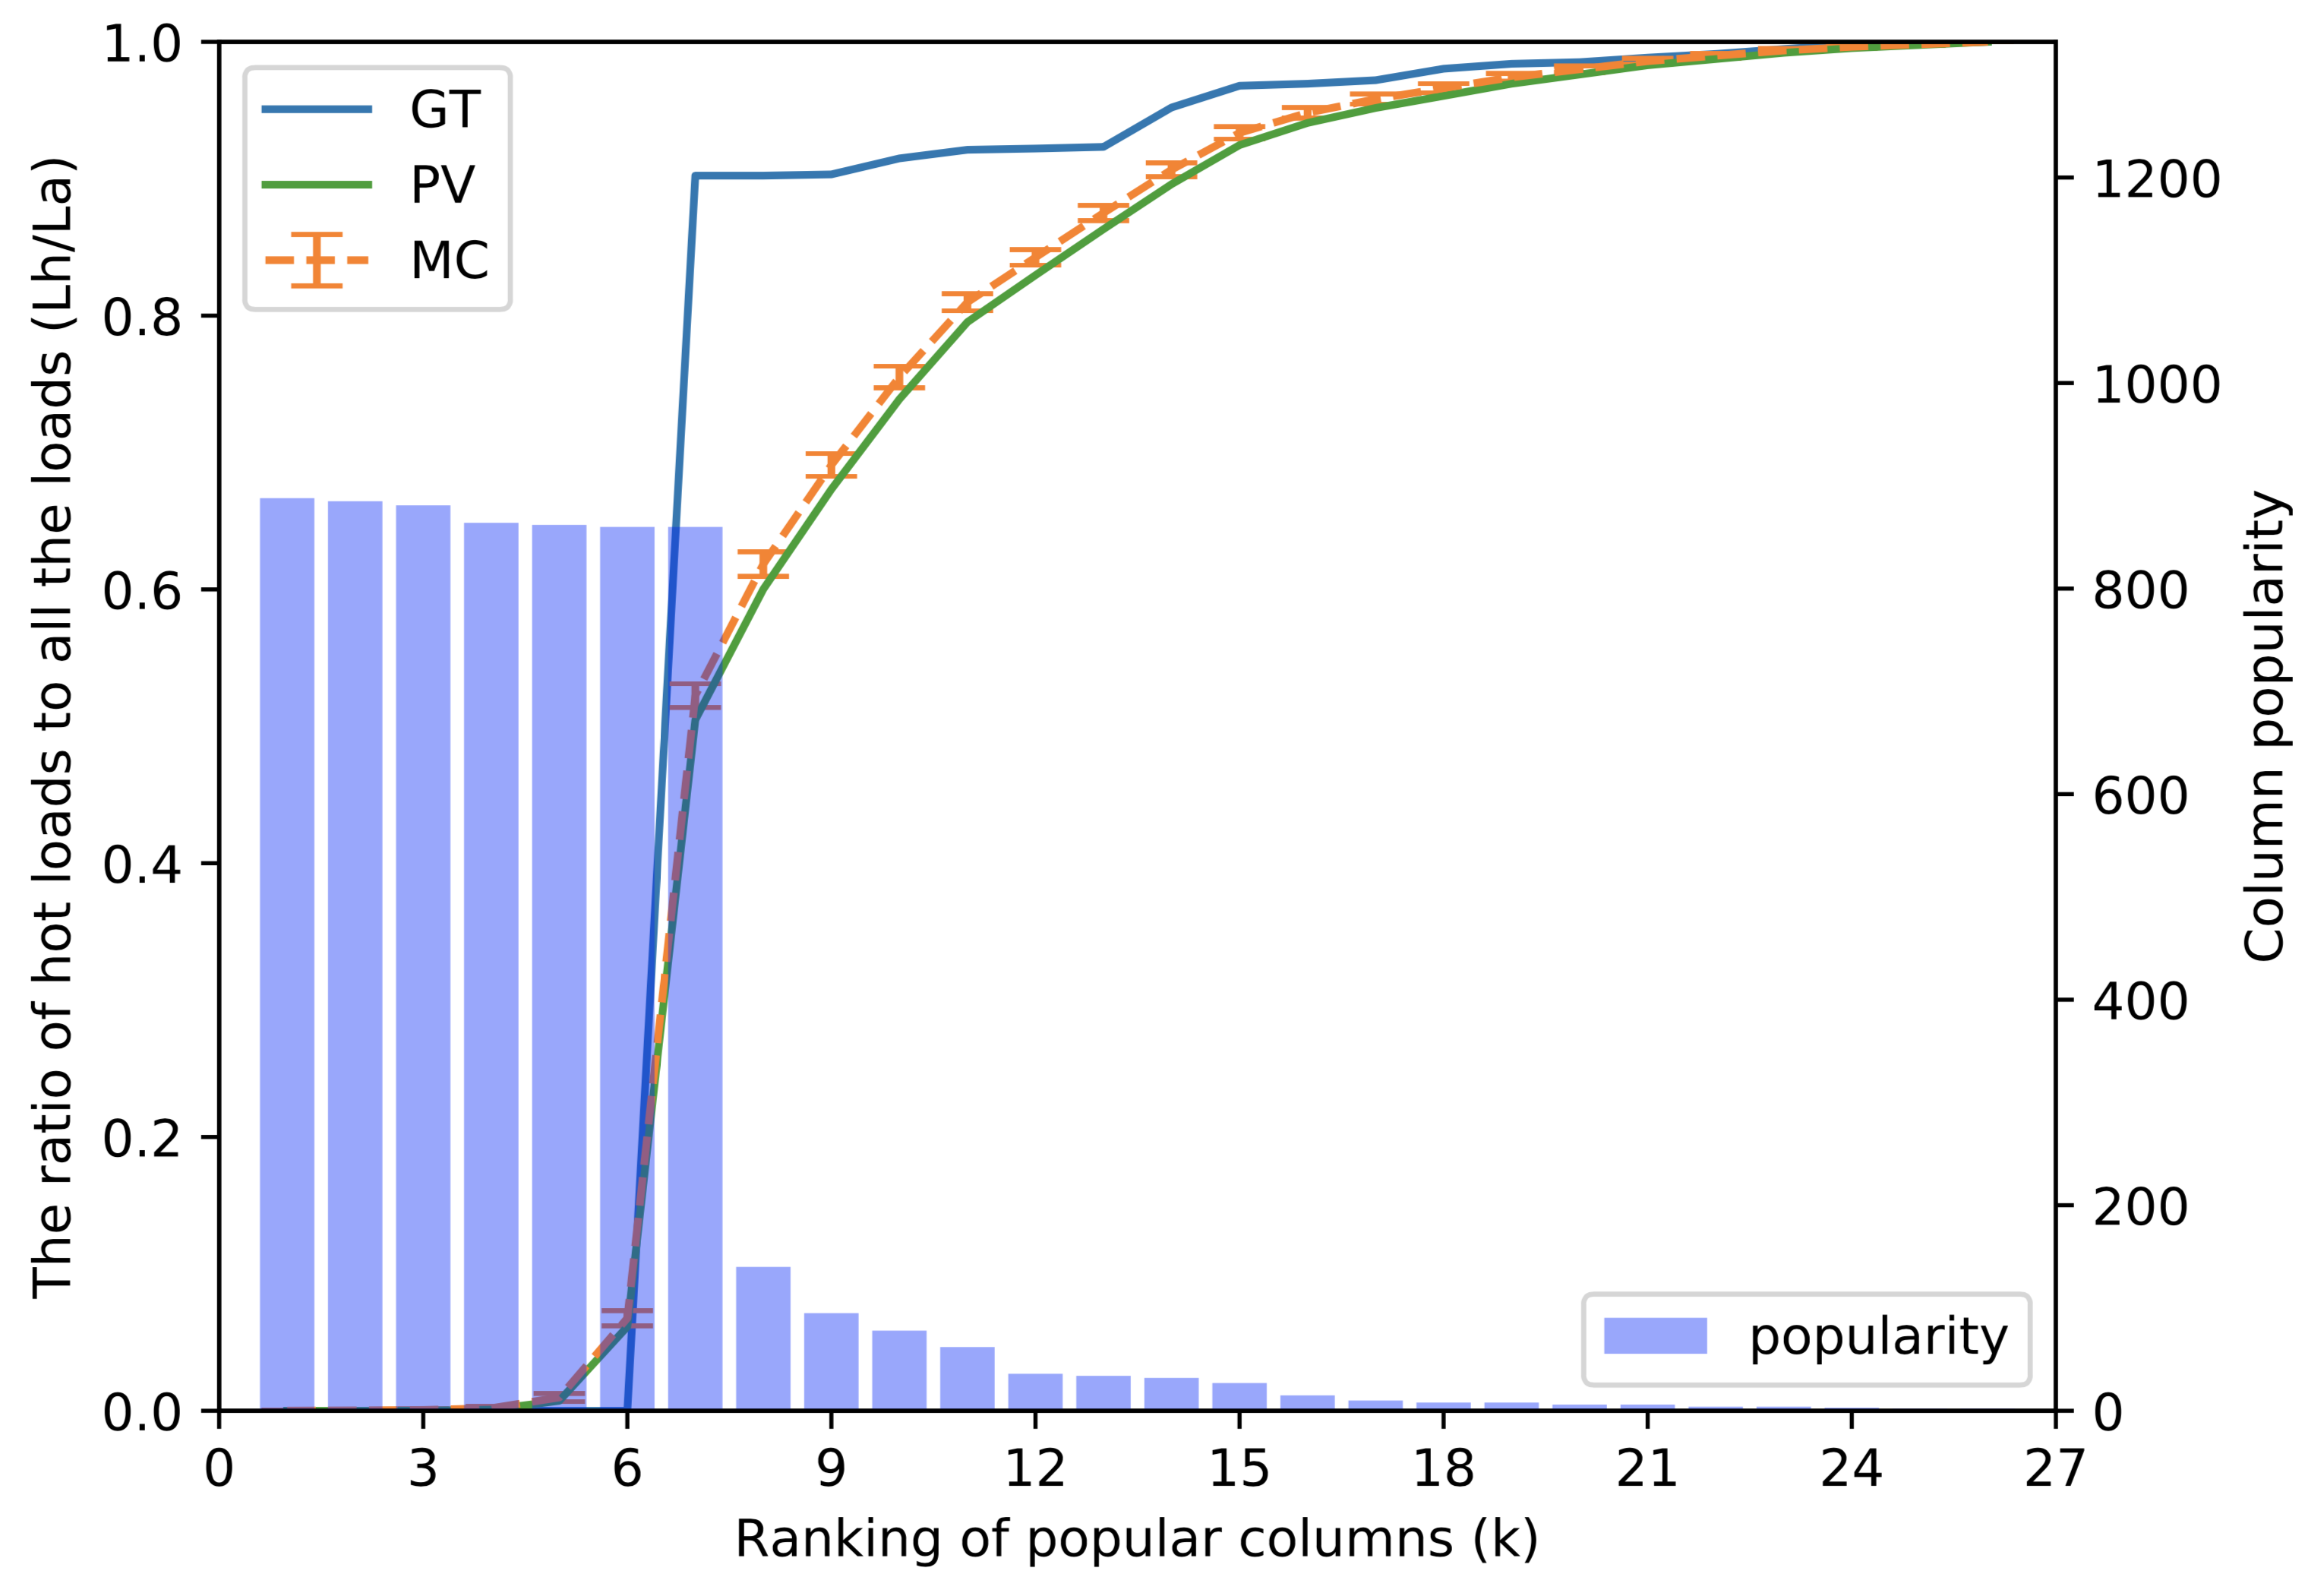
\includegraphics[width=1\textwidth]{img/cw-cache/emul_web_sales}
            \caption{TPC-DS中的 $web\_sales$ 表。}
            \label{fig:emul-ws}
        \end{subfigure}%
        \caption{负载差异大(skewed workloads)的情况下,蒙特卡罗方法、实际值和公式预测值的比较。}
        \label{fig:mc_pv_gt}
        %\vspace{-.1in}
    \end{minipage}
\end{figure}


\par \noindent\textbf{测量实验3} \quad 我们加入了更多测试来验证$L_h$ 和 $k$之间的关系,其中用到的负载热度差异更大。具体来说,不同于之前对TPC-DS标准测试程序提供的查询任务只计数一次,我们对查询任务的热度(数量)进行了配置,使其服从Zipf分布(指数参数设置为2)。这样一来,1) 不同列的热门度差异更大,2) 查询任务的数量更多。图~\ref{fig:mc_pv_gt} 展示了先前提到的3个例子中归一化的$L_h$ 和 $k$之间的关系。根据图中结果,我们发现 1) 因为大部分查询任务只访问很少一部分非常热门的列,大部分的负载可由复制的仅含少部分热门的列的副本承担; 2) 当查询任务的数量增加,通过等式~\ref{equ:lh}预测的$L_h$的值更加接近蒙特卡罗方法得出的值,也就更加接近实际值。


\par 总而言之,经过我们的评估,基于列的热度生成查询任务来估计访问模式的分布是可行的。此外,在列热度分布更加不均衡的情况下进行的测量实验(测量实验3)也启发我们,把前$k$个最热门的列“捆绑”复制是有利可图的。

